% !TeX program = xelatex
\documentclass[12pt,a4paper]{ctexart}

\usepackage[margin=2.5cm]{geometry}
\usepackage{amsmath,amssymb}
\usepackage{booktabs,longtable,multirow}
\usepackage{hyperref}
\usepackage{url}
\usepackage{enumitem}
\usepackage{graphicx}
\usepackage{float}
\usepackage{listings}
\usepackage{xcolor}
\usepackage{tikz}
\usetikzlibrary{arrows,shapes,positioning}

\hypersetup{colorlinks=true, linkcolor=blue, citecolor=blue, urlcolor=blue}
\lstset{
  basicstyle=\ttfamily\small,
  breaklines=true,
  frame=single,
  numbers=left,
  numberstyle=\tiny,
  backgroundcolor=\color{gray!5}
}

\newcommand{\coverfield}[2]{%
  \makebox[5.2cm][l]{\heiti\Large #1：} &
  \underline{\makebox[8.4cm][c]{\Large #2}} \\[0.45cm]
}

\newcommand{\makecoursecover}[1]{%
\begin{titlepage}
\centering
\vspace*{2.2cm}

\includegraphics[width=0.48\textwidth]{figures/fzu_sf.png}\par
\vspace{2.1cm}
{\heiti\fontsize{36pt}{44pt}\selectfont 《机器学习》\par}
\vspace{0.25cm}
{\heiti\fontsize{36pt}{44pt}\selectfont #1\par}
\vspace{2.0cm}
\renewcommand{\arraystretch}{1.2}
\begin{tabular}{rl}
  \makebox[5.2cm][l]{\heiti\Large 题\qquad 目：} &
  \underline{\makebox[8.4cm][c]{\Large 小样本条件下中文多角色}} \\[0.35cm]
  & \underline{\makebox[8.4cm][c]{\Large 文本风格迁移研究}} \\[0.45cm]
  \coverfield{学生姓名（学号）}{王浩楠（102301325）}
  \coverfield{学生姓名（学号）}{张博凇（102301314）}
  \coverfield{学生姓名（学号）}{范智杰（102301340）}
  \coverfield{学生姓名（学号）}{何顺康（102301336）}
  \coverfield{学生姓名（学号）}{陈佳铭（102301539）}
  \coverfield{指 导 教 师}{于元隆、朱丹红}
\end{tabular}
\end{titlepage}
}

\begin{document}
\makecoursecover{科研实训报告}
\newpage
\tableofcontents
\newpage

\section{实验概述}

\subsection{研究背景}

文本风格迁移（Text Style Transfer）旨在保持文本核心语义不变的前提下改变其表达风格。传统风格迁移任务常将风格视作相对单一的标签，例如“正面/负面情感”“正式/非正式”“古风/现代”等。然而在真实中文交流中，风格并不只是语言表层装饰，而是与说话对象、社会关系、礼貌等级和场景预期紧密相关。

例如，原句“我今天加班，可能晚点回去”在不同对象下可改写为：

\begin{itemize}[leftmargin=2em]
  \item 对老板：``今天项目这边还需要多处理一会儿，进度我会及时同步给您。''
  \item 对同事：``我今天可能还要加会儿班，晚点再过去，方便的话你们先开始。''
  \item 对好朋友：``我今天又得加班了，估计晚点到，你们先别等我。''
  \item 对女朋友：``宝贝，我今天要加会儿班，可能晚点回去，忙完马上找你。''
  \item 对母亲：``妈，我今天加班，可能晚点回去，你早点休息，不用等我。''
\end{itemize}

这些句子的事实内容基本一致，但称呼、礼貌程度、情绪表达和信息组织方式存在明显差异。本项目希望使模型学习这种关系感知表达能力：模型不是扮演老板或母亲说话，而是始终以“我”为说话者，根据当前说话对象调整表达方式。

\subsection{研究目标}

本项目的目标包括以下四个方面：

\begin{enumerate}[leftmargin=2em]
  \item \textbf{数据构建：} 从中文对话语料中筛选适合改写的第一人称中性句，利用大语言模型生成五类关系对象下的改写文本，形成可用于监督微调的平行数据。
  \item \textbf{质量控制：} 设计自动质检脚本，对教师数据中的语义漂移、数字丢失、时间信息丢失、模板化改写和角色区分度不足等问题进行标记与过滤。
  \item \textbf{模型训练：} 基于 mT0-large 进行单 LoRA 参数高效微调，利用简洁稳定的指令模板实现角色条件控制。
  \item \textbf{系统实现：} 开发完整 Web 演示系统，支持 DeepSeek 教师模型、微调模型和 baseline 模型的在线对比。
\end{enumerate}

\subsection{小组分工}

\begin{table}[H]
\centering
\caption{成员分工与占比}
\begin{tabular}{p{1.6cm}|p{1.4cm}|p{3cm}|p{6.8cm}}
\toprule
成员 & 分工占比 & 主要职责 & 具体工作内容 \\
\midrule
王浩楠 & 20\% & 项目统筹与核心代码实现 & 参与数据处理、模型训练、后端接口、前端页面、数据库联调和华为云部署等全流程代码编写；同时负责研究问题设计、整体方案统筹、系统整合和报告最终整理。 \\
张博凇 & 20\% & 模型训练与微调 & 负责 mT0-large、LoRA 训练脚本、超参数配置、训练数据格式转换和推理接口适配。 \\
范智杰 & 20\% & 数据构建与质量控制 & 负责 LCCC 数据抽取、DeepSeek 批量改写、自动质检规则设计和过滤后数据集生成。 \\
何顺康 & 20\% & 前端系统开发 & 负责 Vue 3 页面、聊天式交互、五角色对比、多模型对比和历史记录展示。 \\
陈佳铭 & 20\% & 后端与数据库 & 负责 FastAPI 接口、用户鉴权、MySQL 表设计、历史记录存储和模型服务集成。 \\
\bottomrule
\end{tabular}
\end{table}

\subsection{阶段进度安排}

为体现科研实训过程的连续性，项目可按“数据、模型、系统、报告”四条线记录阶段进度。后续可根据实际开发时间补充每周完成内容、遇到的问题和调整原因。

\begin{table}[H]
\centering
\caption{阶段进度安排}
\label{tab:schedule}
\begin{tabular}{p{2.2cm}|p{4.2cm}|p{6.2cm}}
\toprule
阶段 & 主要任务 & 产出材料 \\
\midrule
第 1 阶段 & 任务定义与文献调研 & 明确五类目标对象、确定文本风格迁移和 LoRA 微调路线。 \\
第 2 阶段 & 数据抽取与教师改写 & 中性句数据、DeepSeek 批量改写结果、质量检查脚本。 \\
第 3 阶段 & 模型微调与推理适配 & 训练/验证/测试集、LoRA checkpoint、模型推理接口。 \\
第 4 阶段 & 前后端系统实现 & FastAPI 后端、Vue 前端、MySQL 数据库和演示页面。 \\
第 5 阶段 & 测试、分析与报告整理 & 样例对比、错误案例分析、系统截图和最终报告。 \\
\bottomrule
\end{tabular}
\end{table}

\section{实验数据集}

\subsection{数据来源}

本项目选用 LCCC（Large-scale Cleaned Chinese Conversation）作为原始语料来源。LCCC 是公开中文对话数据集，具有日常表达丰富、口语化程度高、话题覆盖广的特点，适合从中抽取第一人称日常陈述句。与新闻、百科或书面语数据相比，微博对话语料更接近日常即时沟通场景，因此更适合构建关系感知改写任务。

由于原始对话中包含大量无实质内容、情绪强烈、角色已固定或不适合改写的语句，项目首先设计了中性句抽取管线，从原始对话中筛选“语义明确、可对多个对象表达、具有改写空间”的句子。

\subsection{中性句抽取}

中性句抽取脚本位于 \texttt{dataset/extract\_neutral.py}。主要过滤逻辑如下：

\begin{enumerate}[leftmargin=2em]
  \item \textbf{拆句与清洗：} 去除 LCCC 中的空格分词形式，按照中文终止标点切分单句。
  \item \textbf{长度过滤：} 保留 8 到 65 字之间的句子，过短句子信息不足，过长句子容易包含多个事件。
  \item \textbf{角色标记排除：} 排除含“宝贝”“领导”“妈”“老板”等已显式带有角色对象的句子。
  \item \textbf{强情绪和广告排除：} 过滤脏话、营销信息、纯感叹、过多标点和无意义重复。
  \item \textbf{第一人称约束：} 优先保留包含“我”的句子，使任务保持“说话者不变”的设定。
  \item \textbf{信息量评分：} 对包含时间、计划、工作、出行、身体状态等关键词的句子加权排序。
\end{enumerate}

最终得到 2000 条中性候选句，作为教师模型批量改写的输入。

\subsection{教师模型批量改写}

数据生成脚本位于 \texttt{dataset/generate\_rewrites.py}。项目使用 DeepSeek API 作为教师模型，将每条中性句改写为五类目标对象下的表达：

\[
\mathcal{R}=\{\text{老板},\text{同事},\text{好朋友},\text{女朋友},\text{母亲}\}
\]

生成时明确要求模型保持核心语义不变，不新增原句未出现的事实信息，不改变时间、地点、人物、数量和因果关系。对于明显不适合对某一对象表达的内容，允许输出 \texttt{N/A}。批量生成采用 JSON Array 格式，便于后续解析和质量检查。

\subsection{数据质量控制}

教师模型生成的数据并非天然可靠。常见问题包括：

\begin{itemize}[leftmargin=2em]
  \item 为了使表达自然而新增承诺，例如原句只说“晚点回去”，输出却增加“忙完马上找你”。
  \item 数字或时间信息丢失，例如原句包含“80 多斤”“今天”“明天”，改写中被省略。
  \item 角色风格模板化，例如女朋友角色大量使用“宝贝”，母亲角色大量使用“妈，别担心”。
  \item 五个角色之间差异不足，只有称呼变化，句式和语气几乎相同。
\end{itemize}

因此项目新增 \texttt{dataset/quality\_filter.py}，从以下维度进行自动质检：

\begin{table}[H]
\centering
\caption{数据质检规则}
\begin{tabular}{p{4cm}|p{8.5cm}}
\toprule
规则 & 作用 \\
\midrule
长度阈值 & 过滤过短、过长或与原句长度比例异常的输出。 \\
数字一致性 & 若原句包含数字，改写中应保留对应数字。 \\
时间关键词一致性 & 检查“今天、明天、晚上、周末”等时间信息是否丢失。 \\
ROUGE-L 相似度 & 相似度过低可能语义漂移；相似度过高则提示改写不足。 \\
模板词检测 & 检查是否只是添加“宝贝、妈、您”等模板词。 \\
角色间相似度 & 标记不同角色输出过于相似的样本，供后续二次生成。 \\
\bottomrule
\end{tabular}
\end{table}

过滤后数据统计如表~\ref{tab:data_stats} 所示。质检采用角色级过滤，即某条样本中某一角色不合格时仅将该角色置为 \texttt{N/A}，保留其他可用角色，最大限度减少数据浪费。

\begin{table}[H]
\centering
\caption{过滤后数据统计}
\label{tab:data_stats}
\begin{tabular}{c|c}
\toprule
项目 & 数量 \\
\midrule
原始中性句 & 2000 \\
保留样本条目 & 1966 \\
有效角色改写 & 8957 \\
过滤角色改写 & 1043 \\
训练集 & 7165 \\
验证集 & 895 \\
测试集 & 897 \\
\bottomrule
\end{tabular}
\end{table}

\subsection{数据样例与问题样例}

为了说明数据构建的实际效果，表~\ref{tab:data_example} 给出一条“原句--五角色改写”样例。相比只给出总数，样例能够更直观地说明本项目希望模型学习的关系化表达差异。

\begin{table}[H]
\centering
\caption{数据构建样例}
\label{tab:data_example}
\begin{tabular}{p{2.4cm}|p{9.8cm}}
\toprule
字段 & 内容 \\
\midrule
原句 & 我今天加班，可能晚点回去。 \\
老板 & 今天项目这边还需要多处理一会儿，进度我会及时同步给您。 \\
同事 & 我今天可能还要加会儿班，晚点再过去，方便的话你们先开始。 \\
好朋友 & 我今天又得加班了，估计晚点到，你们先别等我。 \\
女朋友 & 宝贝，我今天要加会儿班，可能晚点回去，忙完马上找你。 \\
母亲 & 妈，我今天加班，可能晚点回去，你早点休息，不用等我。 \\
\bottomrule
\end{tabular}
\end{table}

教师模型生成的数据并非全部可直接用于训练。表~\ref{tab:bad_teacher_examples} 总结了质检阶段重点关注的低质量类型，这些问题会影响模型对事实保持和角色表达的学习，因此需要在训练前进行过滤。

\begin{table}[H]
\centering
\caption{低质量教师数据类型}
\label{tab:bad_teacher_examples}
\begin{tabular}{p{3cm}|p{4cm}|p{5cm}}
\toprule
问题类型 & 表现形式 & 分析说明 \\
\midrule
数字丢失 & 改写后删除或改变原句中的数字 & 数字通常对应时间、数量或计划安排，丢失后会直接改变事实。 \\
时间丢失 & 遗漏今天、明天、晚上等时间词 & 时间信息是日常沟通中的关键约束，不能为了语气变化而省略。 \\
语义漂移 & 新增承诺、原因或结果 & 改写结果扩大了原句事实范围，容易造成误导。 \\
模板化改写 & 只添加称呼词，正文几乎不变 & 角色差异停留在表层称呼，无法提供有效训练信号。 \\
角色不适配 & 对老板过于随意，或对亲密对象过于工作汇报式 & 输出虽然通顺，但不符合目标对象的关系预期。 \\
\bottomrule
\end{tabular}
\end{table}

\section{理论基础}

\subsection{文本风格迁移}

文本风格迁移可形式化为：给定源文本 $x$ 和目标风格条件 $s$，生成文本 $y=G_\theta(x,s)$，要求 $y$ 在语义上保持 $x$ 的核心内容，同时在风格上符合 $s$。本项目中的风格条件并非单一情感或正式度标签，而是由说话对象及其社会关系共同决定。

与传统风格迁移相比，本任务具有三个特点：

\begin{enumerate}[leftmargin=2em]
  \item \textbf{角色条件细粒度：} 五类对象不仅正式度不同，还涉及权力差、亲密距离和场景领域。
  \item \textbf{语义保持要求强：} 日常沟通中时间、数量、人物、计划等信息不能随意改变。
  \item \textbf{输出自然性要求高：} 改写不能只替换称呼，而应符合真实中文表达习惯。
\end{enumerate}

\subsection{mT0 与指令式输入}

mT0 是在 mT5 基础上经过多任务指令微调的多语言 Seq2Seq 模型。相较于 mT5，mT0 更适合处理“任务说明+输入+输出”的文本到文本任务。本项目采用如下短指令格式：

\begin{lstlisting}[language={},caption={mT0 输入模板}]
任务：保持原意，按目标对象改写语气。
对象：女朋友
风格：亲密、温柔、在意对方感受
原句：我今天加班，可能晚点回去
改写：
\end{lstlisting}

该模板相比长篇规则说明更稳定：字段少、结构固定、角色信息明确，同时不会占用过多输入长度。训练和后端推理使用完全一致的模板，避免训练-推理分布不一致。

\subsection{LoRA 参数高效微调}

LoRA（Low-Rank Adaptation）通过在 Transformer 权重更新中引入低秩矩阵分解来减少可训练参数。对于原始权重矩阵 $W$，LoRA 不直接更新 $W$，而是学习低秩增量：

\[
W' = W + \Delta W,\quad \Delta W = BA
\]

其中 $A$ 和 $B$ 的秩远小于原矩阵维度。这样既保留了预训练模型的语言能力，又能以较低显存和存储成本适配下游任务。

\subsection{单 LoRA 与多 LoRA 方案选择}

项目初期考虑过“每个角色一个 LoRA 适配器”的方案，即分别为老板、同事、好朋友、女朋友和母亲训练独立适配器。这种方案结构直观，但并不适合本项目的小样本条件。过滤后有效角色改写总数为 8957 条，若拆分为五个独立 LoRA，每个角色只能使用约一千余条样本，容易学习到“您”“宝贝”“妈”等表层模板词，而难以稳定学习语义保持、句式重组和自然表达能力。

因此，本项目最终采用“单 LoRA + 角色条件输入”的方案。所有角色样本共享同一个 LoRA 适配器，模型在统一数据中学习通用的中文改写能力和事实保持能力，再通过输入模板中的“对象”和“风格”字段控制输出方向。该方案有四点优势：第一，扩大了每次训练可利用的数据规模，降低单角色过拟合风险；第二，使不同角色共享语义保持、时间数字保留和自然改写等公共能力；第三，部署时只需加载一个适配器，存储和推理管理更简单；第四，训练模板与后端推理模板保持一致，便于在 Web 系统中通过角色参数直接切换输出风格。对于本项目这种五类角色、数据规模有限、需要系统演示的场景，单 LoRA 条件模型比多 LoRA 方案更稳妥。

\section{模型设计与实验过程}

\subsection{整体流程}

项目整体流程如图~\ref{fig:pipeline} 所示。

\begin{figure}[H]
\centering
\begin{tikzpicture}[node distance=1.7cm, auto, >=latex']
  \tikzstyle{block}=[rectangle, draw, rounded corners, align=center, minimum height=0.9cm, minimum width=2.8cm]
  \node[block] (raw) {LCCC 原始对话};
  \node[block, right=of raw] (neutral) {中性句抽取};
  \node[block, right=of neutral] (teacher) {DeepSeek 教师改写};
  \node[block, below=of teacher] (filter) {质量过滤};
  \node[block, left=of filter] (data) {mT0 指令数据};
  \node[block, left=of data] (train) {单 LoRA 微调};
  \node[block, below=of data] (system) {Web 演示系统};
  \draw[->] (raw) -- (neutral);
  \draw[->] (neutral) -- (teacher);
  \draw[->] (teacher) -- (filter);
  \draw[->] (filter) -- (data);
  \draw[->] (data) -- (train);
  \draw[->] (train) -- (system);
  \draw[->] (filter) -- (system);
\end{tikzpicture}
\caption{项目整体技术流程}
\label{fig:pipeline}
\end{figure}

\subsection{训练数据格式}

过滤后的 \texttt{role\_rewrite\_filtered.jsonl} 被转换为统一训练集，每条样本包含角色代码、角色中文名、原句、模型输入和目标输出。示例如下：

\begin{lstlisting}[language={},caption={训练样本格式}]
{
  "role_code": "mother",
  "role_name": "母亲",
  "source": "我今天加班，可能晚点回去",
  "input": "任务：保持原意，按目标对象改写语气。\n对象：母亲\n风格：尊重、温暖、让长辈放心\n原句：我今天加班，可能晚点回去\n改写：",
  "output": "妈，我今天加班，可能晚点回去，你早点休息，不用等我。"
}
\end{lstlisting}

\subsection{训练配置}

\begin{table}[H]
\centering
\caption{LoRA 微调配置}
\begin{tabular}{c|c}
\toprule
项目 & 配置 \\
\midrule
基座模型 & mT0-large \\
训练方式 & 单 LoRA 适配器 \\
任务形式 & Seq2Seq 文本生成 \\
最大输入长度 & 256 \\
最大输出长度 & 128 \\
LoRA rank & 16 \\
LoRA alpha & 32 \\
LoRA dropout & 0.1 \\
学习率 & $5\times10^{-5}$ \\
训练轮数 & 8 \\
batch size & 8 \\
梯度累积步数 & 1 \\
训练精度 & bf16 \\
训练/验证/测试样本数 & 7165 / 895 / 897 \\
\bottomrule
\end{tabular}
\end{table}

模型训练脚本位于 \path{finetune/train_lora.py}。本次训练命令为：

\begin{lstlisting}[language={},caption={LoRA 微调命令}]
python train_lora.py --epochs 8 --batch-size 8 --grad-accum-steps 1 --lr 5e-5 --lora-r 16 --lora-alpha 32
\end{lstlisting}

训练完成后适配器保存至 \path{finetune/output/final/}，后端推理服务加载 mT0-large 基座模型和该 LoRA 适配器。训练过程日志、损失曲线和测试集预测结果分别保存于 \path{finetune/output/artifacts/} 和 \path{finetune/output/predictions/}。

\subsection{训练过程记录}

正式微调完成后，训练脚本会在 \path{finetune/output/artifacts/} 下保存训练过程材料。其中报告优先使用 \path{train_eval_loss_curve.png}，该图同时展示训练集 loss 和验证集 loss，能够观察模型是否正常收敛，以及验证集损失是否出现明显反弹。若训练 loss 持续下降而验证 loss 同步下降或保持稳定，说明模型没有出现明显过拟合；若训练 loss 下降但验证 loss 上升，则需要考虑提前停止、降低训练轮数或加强数据清洗。

\begin{figure}[H]
\centering
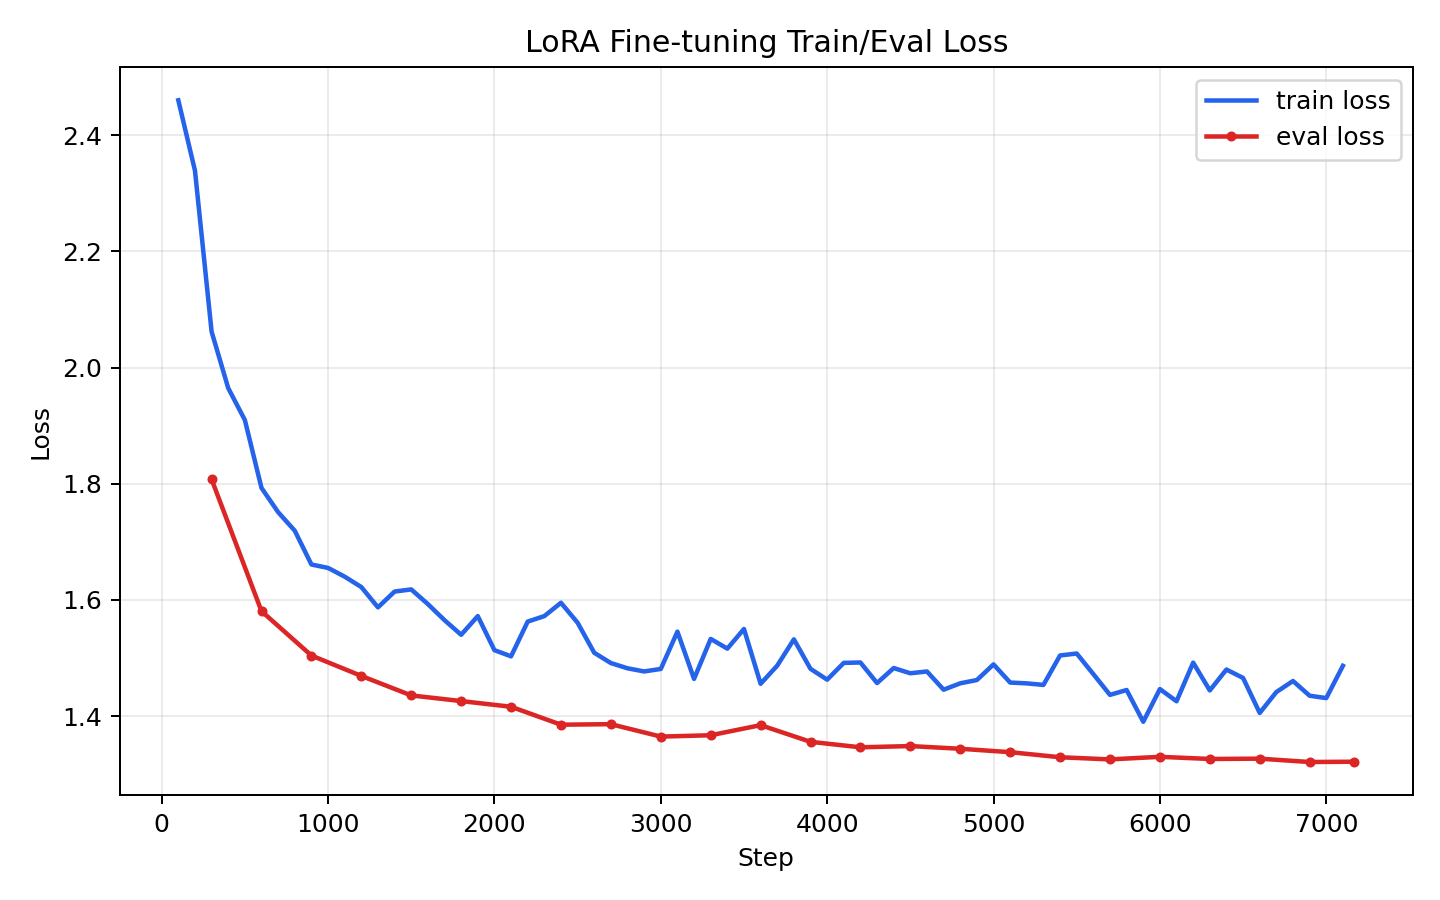
\includegraphics[width=0.85\textwidth]{figures/train_eval_loss_curve.png}
\caption{LoRA 微调训练集与验证集损失曲线}
\label{fig:train_eval_loss_curve}
\end{figure}

从图~\ref{fig:train_eval_loss_curve} 可以看出，训练集损失在前期下降较快，随后进入较平稳的下降阶段；验证集损失整体也保持下降趋势，未出现训练损失下降而验证损失明显反弹的情况。最终在测试集上得到的 \texttt{eval\_loss} 为 1.2962，最优验证指标对应的 checkpoint 为 \path{output/checkpoint-6900}。这说明在当前数据规模下，单 LoRA 条件模型能够学习到主要的角色改写映射关系，同时没有出现明显过拟合迹象。

\subsection{实验中的主要问题与处理}

\begin{enumerate}[leftmargin=2em]
  \item \textbf{教师数据模板化：} DeepSeek 在亲密角色中倾向使用固定称呼。处理方式是在质检脚本中统计模板词，并过滤“只加称呼、正文几乎未改”的样本。
  \item \textbf{语义漂移：} 教师模型可能新增承诺或省略关键信息。处理方式是检查数字、时间关键词和文本相似度。
  \item \textbf{多 LoRA 数据不足：} 初始方案每个角色单独训练 LoRA，但单角色样本量有限。处理方式是改为单 LoRA 条件模型，共享所有角色数据。
  \item \textbf{输入模板冗长：} 过长提示会挤占原句空间，也可能使模型学习不稳定。处理方式是将模板压缩为“任务、对象、风格、原句、改写”五行。
\end{enumerate}

\subsection{对比实验设计}

为了增强实验结果的可解释性，本项目设置了不同模型和不同角色之间的对比思路。对比对象包括 DeepSeek 教师模型、mT0-LoRA 微调模型和规则 baseline 模型，重点观察语义保持、角色适配、自然流畅和角色区分四个方面。

\begin{table}[H]
\centering
\caption{对比实验设置}
\label{tab:comparison_setting}
\begin{tabular}{p{3cm}|p{4.5cm}|p{5cm}}
\toprule
对比对象 & 目的 & 预期观察点 \\
\midrule
DeepSeek vs mT0-LoRA & 比较教师模型和学生模型效果 & LoRA 模型是否能在较低部署成本下学习主要角色表达模式。 \\
mT0-LoRA vs baseline & 验证微调是否有效 & baseline 是否存在输出僵硬、角色差异弱或事实保持差的问题。 \\
五角色横向对比 & 观察同一语义在不同对象下的变化 & 是否不仅改变称呼，还改变语气、信息重点和礼貌程度。 \\
不同输入类型对比 & 检查模型泛化稳定性 & 工作、生活、身体状态、出行计划等场景下表现是否一致。 \\
\bottomrule
\end{tabular}
\end{table}

\section{系统设计与实现}

\subsection{后端架构}

后端采用 FastAPI，主要模块包括：

\begin{itemize}[leftmargin=2em]
  \item \texttt{/api/auth}：注册、登录、JWT 鉴权。
  \item \texttt{/api/meta}：返回角色列表和模型列表。
  \item \texttt{/api/transfers}：接收改写请求，调用模型服务并写入历史记录。
  \item \texttt{/api/accepted-samples}：保存用户采纳的高质量改写结果，供管理员查看和后续整理。
  \item \texttt{/api/users}：管理员查看用户信息。
\end{itemize}

模型服务位于 \texttt{backend/app/services/model\_runner.py}，统一封装三类推理方式：

\begin{enumerate}[leftmargin=2em]
  \item \textbf{DeepSeek API：} 教师模型，也可作为在线对比基准。
  \item \textbf{mT0-LoRA：} 本项目训练得到的单 LoRA 微调模型。
  \item \textbf{规则 baseline：} 基于角色称呼和固定前后缀模板的规则改写方法。
\end{enumerate}

\subsection{数据库设计}

数据库采用 MySQL，核心表结构如表~\ref{tab:database} 所示。

\begin{table}[H]
\centering
\caption{数据库核心表}
\label{tab:database}
\begin{tabular}{c|p{8.5cm}}
\toprule
表名 & 说明 \\
\midrule
\texttt{users} & 用户信息，包含用户名、姓名、密码哈希、管理员标记和账号状态。 \\
\texttt{role\_options} & 目标对象选项，包含角色代码、名称和描述。 \\
\texttt{model\_options} & 模型选项，包含 DeepSeek、baseline 和 LoRA 微调模型。 \\
\texttt{transfer\_records} & 改写历史，记录用户、角色、模型、原句、改写结果和时间。 \\
\texttt{accepted\_samples} & 采纳样本池，保存用户认可的改写结果，用于后续人工审核和增量训练数据整理。 \\
\bottomrule
\end{tabular}
\end{table}

\subsection{前端功能}

前端采用 Vue 3 + Vite，界面采用聊天式布局，并在后续迭代中加入更适合科研展示的对比功能：

\begin{itemize}[leftmargin=2em]
  \item \textbf{单次改写：} 选择一个目标对象和一个模型，生成单条改写结果。
  \item \textbf{五角色对比：} 同一句话同时生成五类对象的改写结果，展示角色差异。
  \item \textbf{多模型对比：} 同一句话在同一目标对象下比较不同模型输出。
  \item \textbf{示例输入：} 提供典型测试句，便于演示和复现实验。
  \item \textbf{历史记录：} 左侧展示用户历史改写结果，便于回看和比较。
  \item \textbf{采纳样本：} 用户可采纳质量较高的改写结果，管理员可查看采纳样本池。
\end{itemize}

\subsection{用户反馈与样本采集}

为了使系统具备后续持续优化能力，项目在演示平台中加入了轻量级用户反馈机制。用户在查看模型生成的改写结果后，可以对认为质量较高的结果进行“采纳”。系统会将被采纳的样本保存到候选训练样本表中，记录原句、目标对象、模型类型、改写结果、采纳用户和创建时间等信息。管理员可以在后台查看采纳样本池，用于后续人工复核和数据整理。

该机制并不直接触发线上自动训练，而是作为增量数据沉淀入口。这样可以避免未经审核的用户反馈直接进入训练集，降低噪声样本对模型的影响。当采纳样本积累到一定规模后，工作人员可以筛选高质量样本，并导出为与现有 LoRA 训练数据一致的格式，再通过离线训练脚本继续微调模型。由此，系统可以形成“模型生成--用户采纳--人工审核--增量训练--模型更新”的持续优化闭环。

\subsection{接口与功能测试}

系统实现完成后，需要对核心接口和前端功能进行测试。后续可在本节补充接口请求示例、返回字段、测试截图和异常处理情况。

\begin{table}[H]
\centering
\caption{后端接口测试项}
\label{tab:api_tests}
\begin{tabular}{p{4.2cm}|p{2.8cm}|p{5.2cm}}
\toprule
接口 & 测试目标 & 预期结果 \\
\midrule
\path{/api/auth/login} & 登录鉴权 & 正确账号返回 token，错误账号返回错误信息。 \\
\path{/api/meta/roles} & 角色列表 & 返回老板、同事、好朋友、女朋友、母亲五类对象。 \\
\path{/api/meta/models} & 模型列表 & 返回 DeepSeek、mT0-LoRA、baseline 等可选模型。 \\
\path{/api/transfers} & 单次改写 & 返回目标角色下的改写文本，并写入历史记录。 \\
\path{/api/transfers/history} & 历史记录 & 返回当前用户历史改写结果，支持前端展示。 \\
\path{/api/accepted-samples} & 点赞样本 & 保存用户点赞的改写结果，进入管理员待审核样本池。 \\
\path{/api/accepted-samples/export} & 数据导出 & 管理员下载已采纳入库的高质量样本，用于后续二次训练。 \\
\bottomrule
\end{tabular}
\end{table}

\subsection{系统截图与部署展示}

为说明本项目不仅完成了离线数据构建和模型微调，也实现了可交互的 Web 演示系统，本节补充系统主要页面截图。截图覆盖用户认证、文本改写、多角色对比、多模型对比、用户点赞、管理员审核、数据导出和服务器部署等环节，能够从工程侧支撑“数据--模型--系统--反馈”的完整闭环。

\begin{figure}[H]
\centering
\begin{minipage}{0.48\textwidth}
\centering
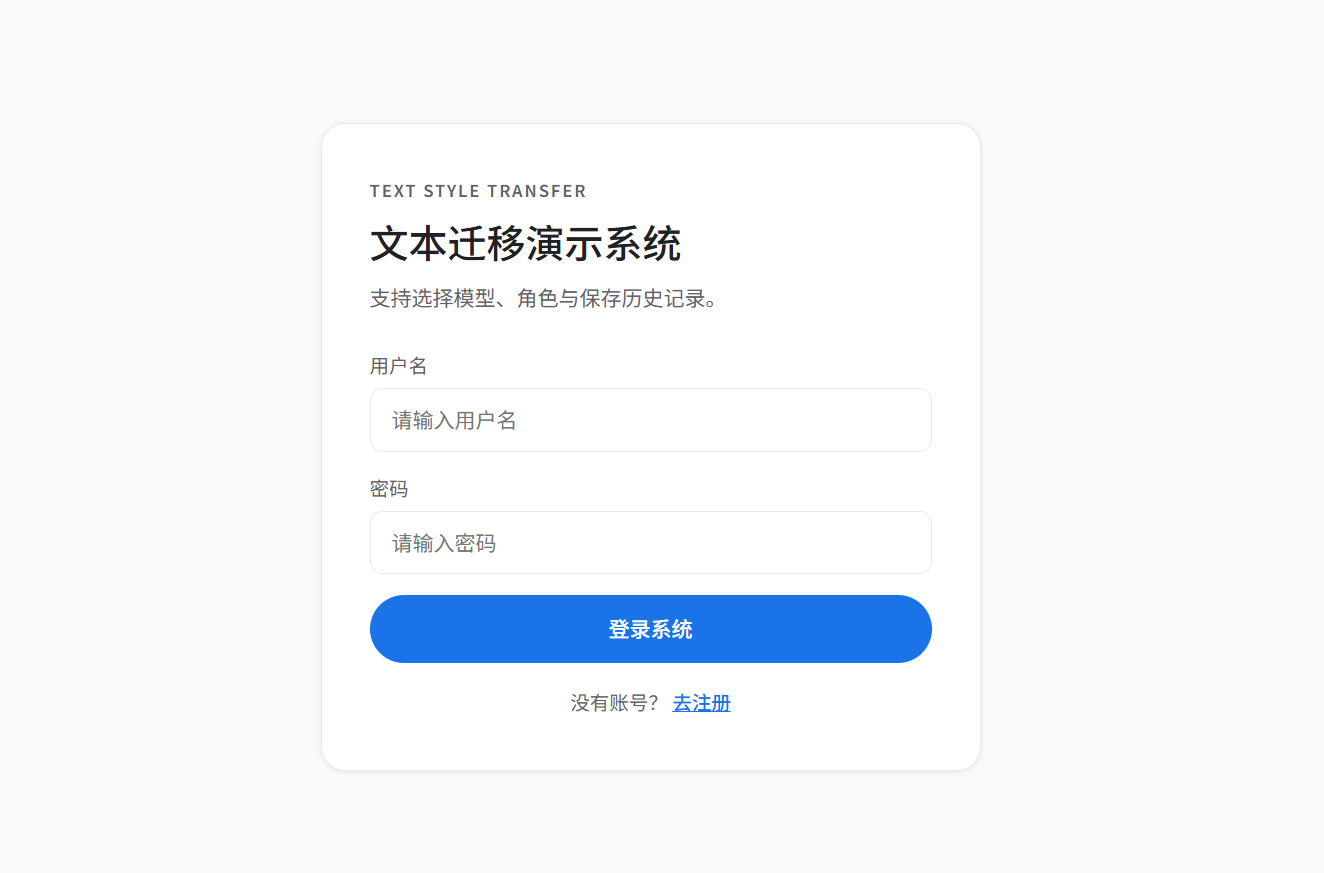
\includegraphics[width=\textwidth]{figures/login.png}
\caption{系统登录页面}
\label{fig:login_page}
\end{minipage}
\hfill
\begin{minipage}{0.48\textwidth}
\centering
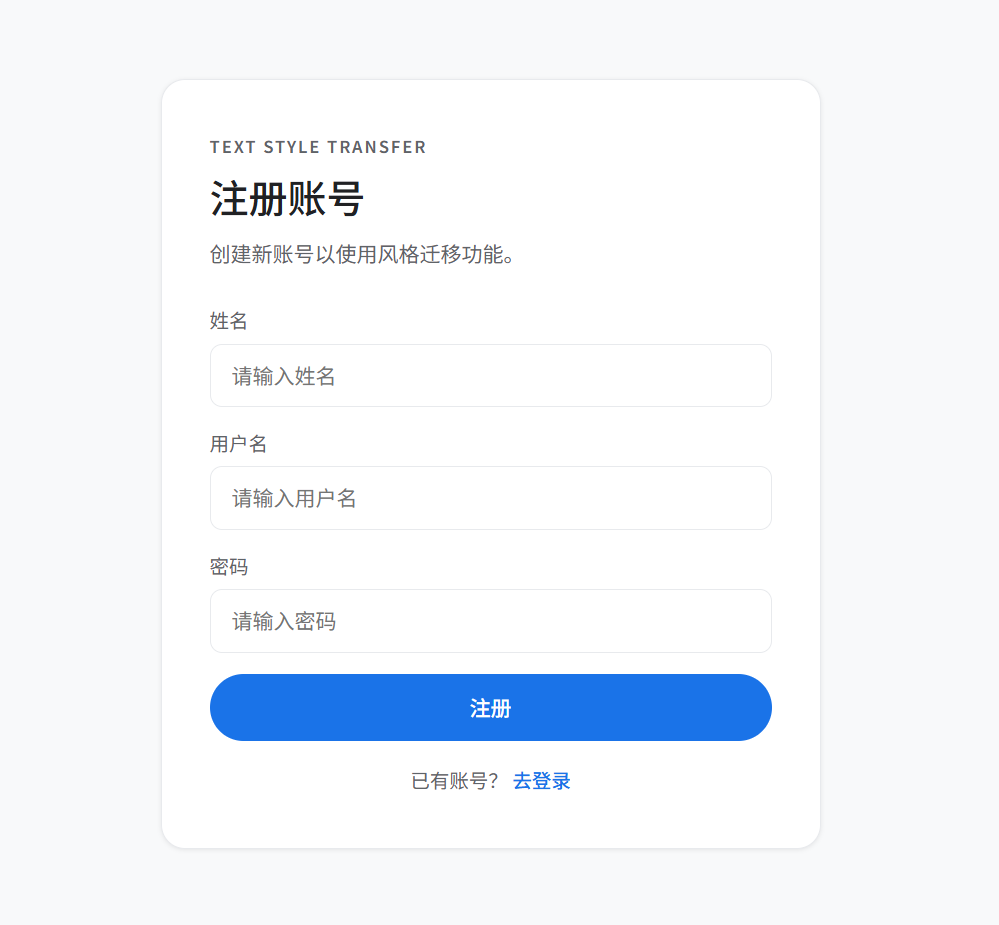
\includegraphics[width=\textwidth]{figures/register.png}
\caption{系统注册页面}
\label{fig:register_page}
\end{minipage}
\end{figure}

\begin{figure}[H]
\centering
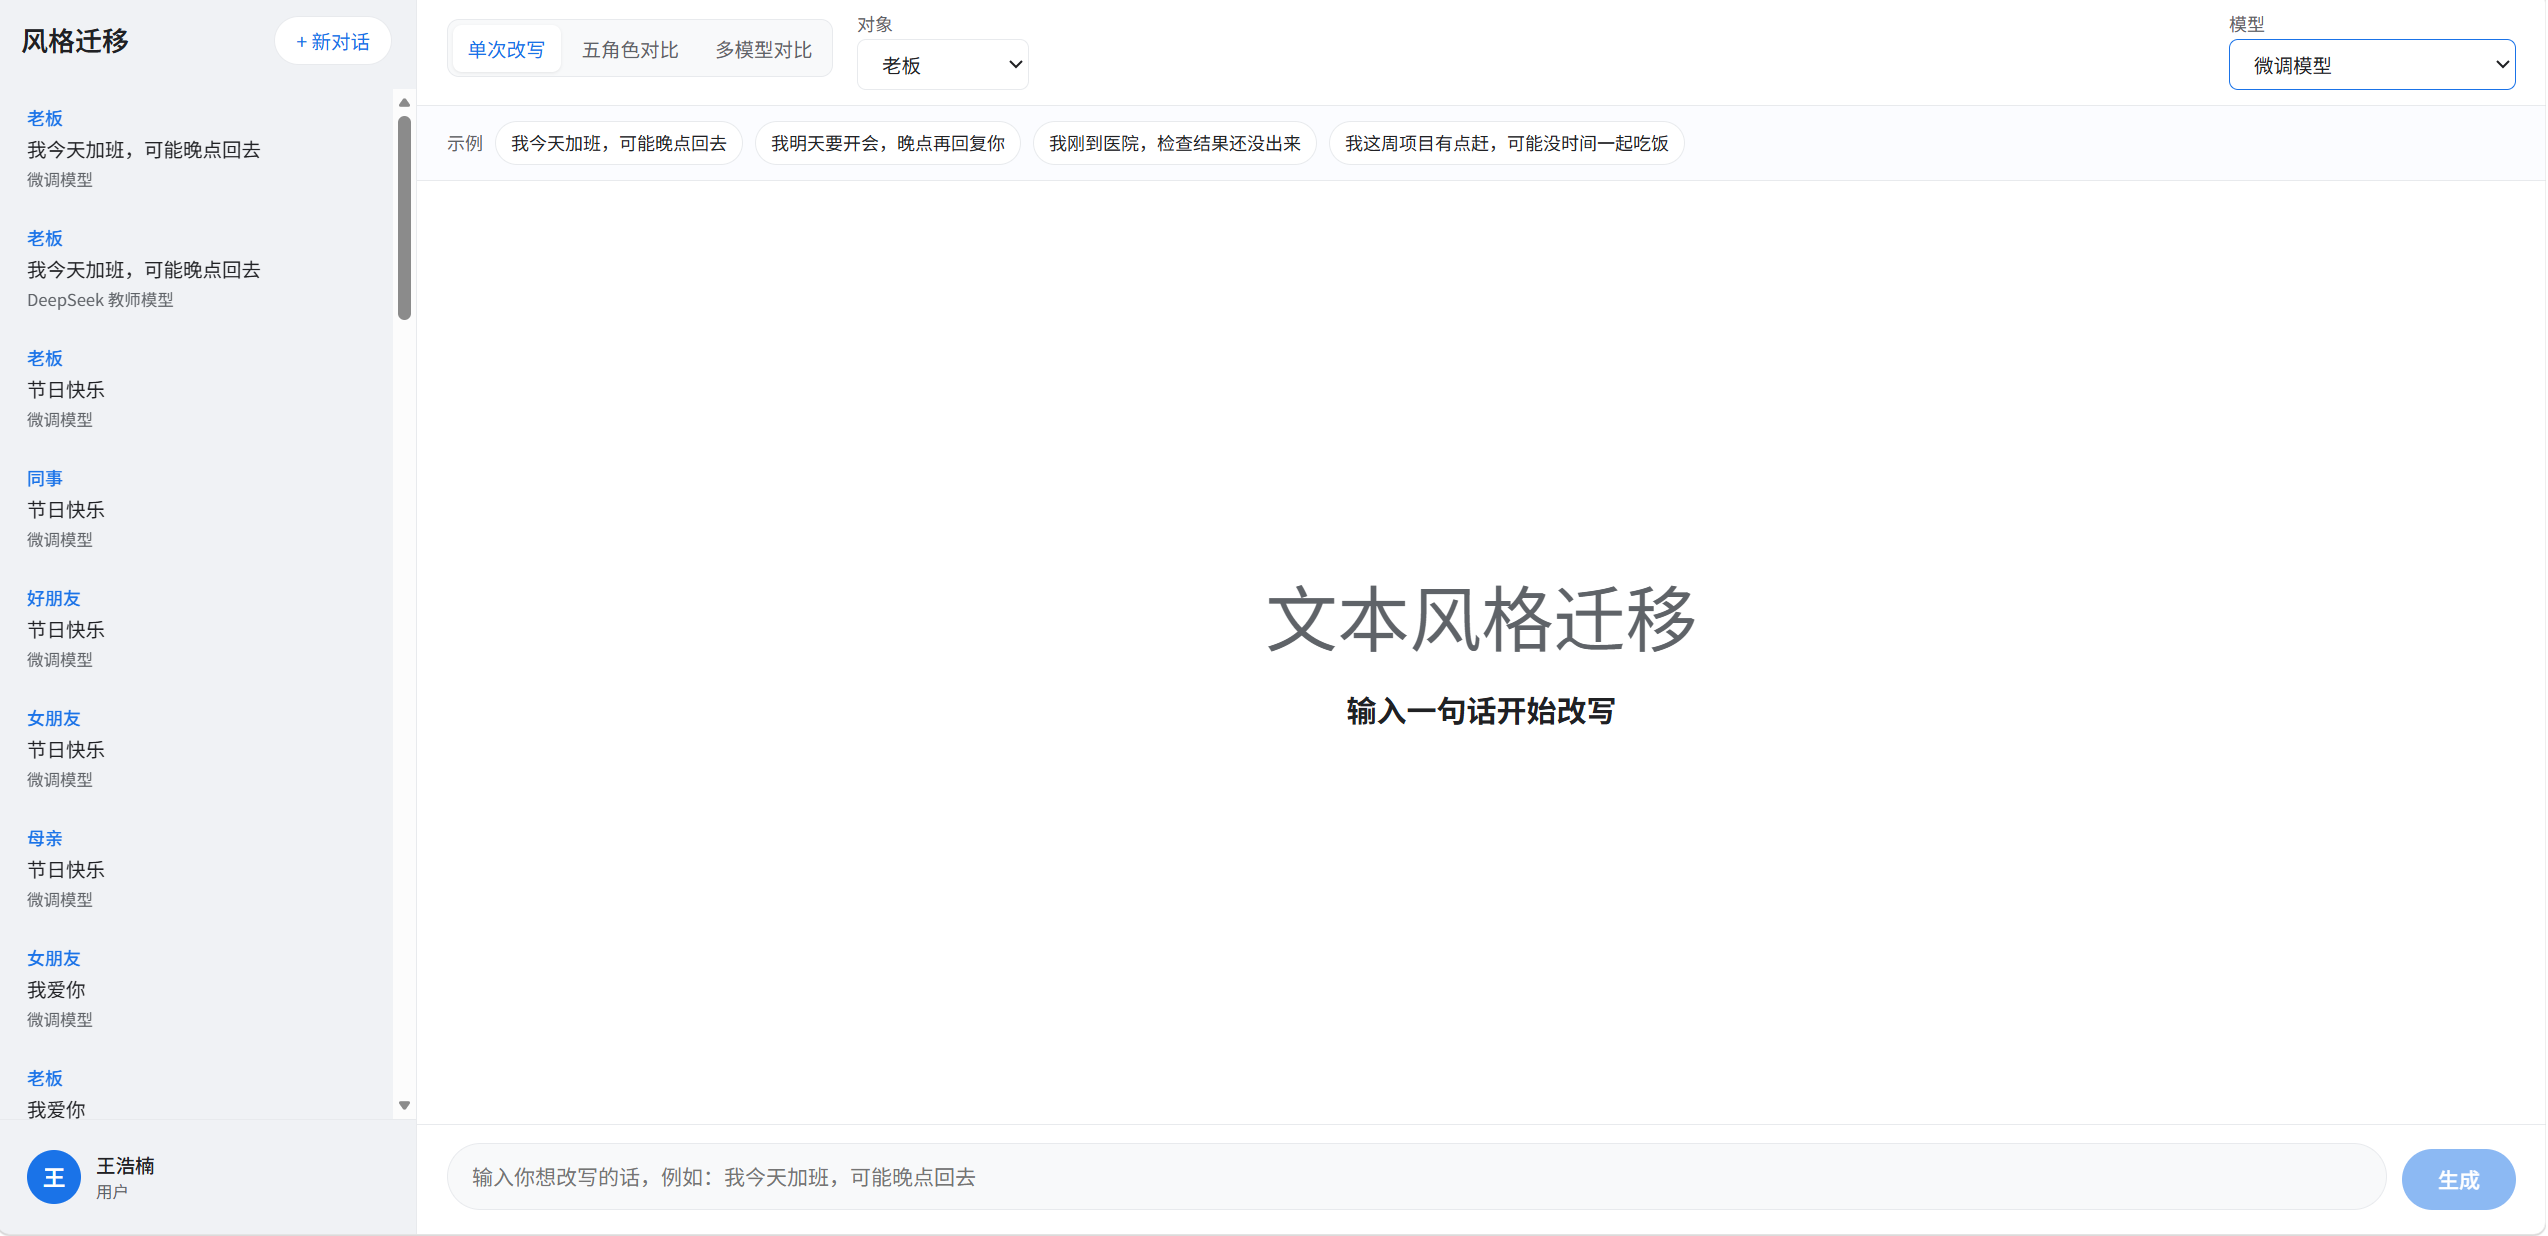
\includegraphics[width=0.9\textwidth]{figures/main_user.png}
\caption{普通用户主界面}
\label{fig:main_user_page}
\end{figure}

图~\ref{fig:login_page} 和图~\ref{fig:register_page} 展示了系统的用户认证入口。用户登录后进入图~\ref{fig:main_user_page} 所示主界面，可选择目标对象、模型类型和改写模式，并查看历史记录。

\begin{figure}[H]
\centering
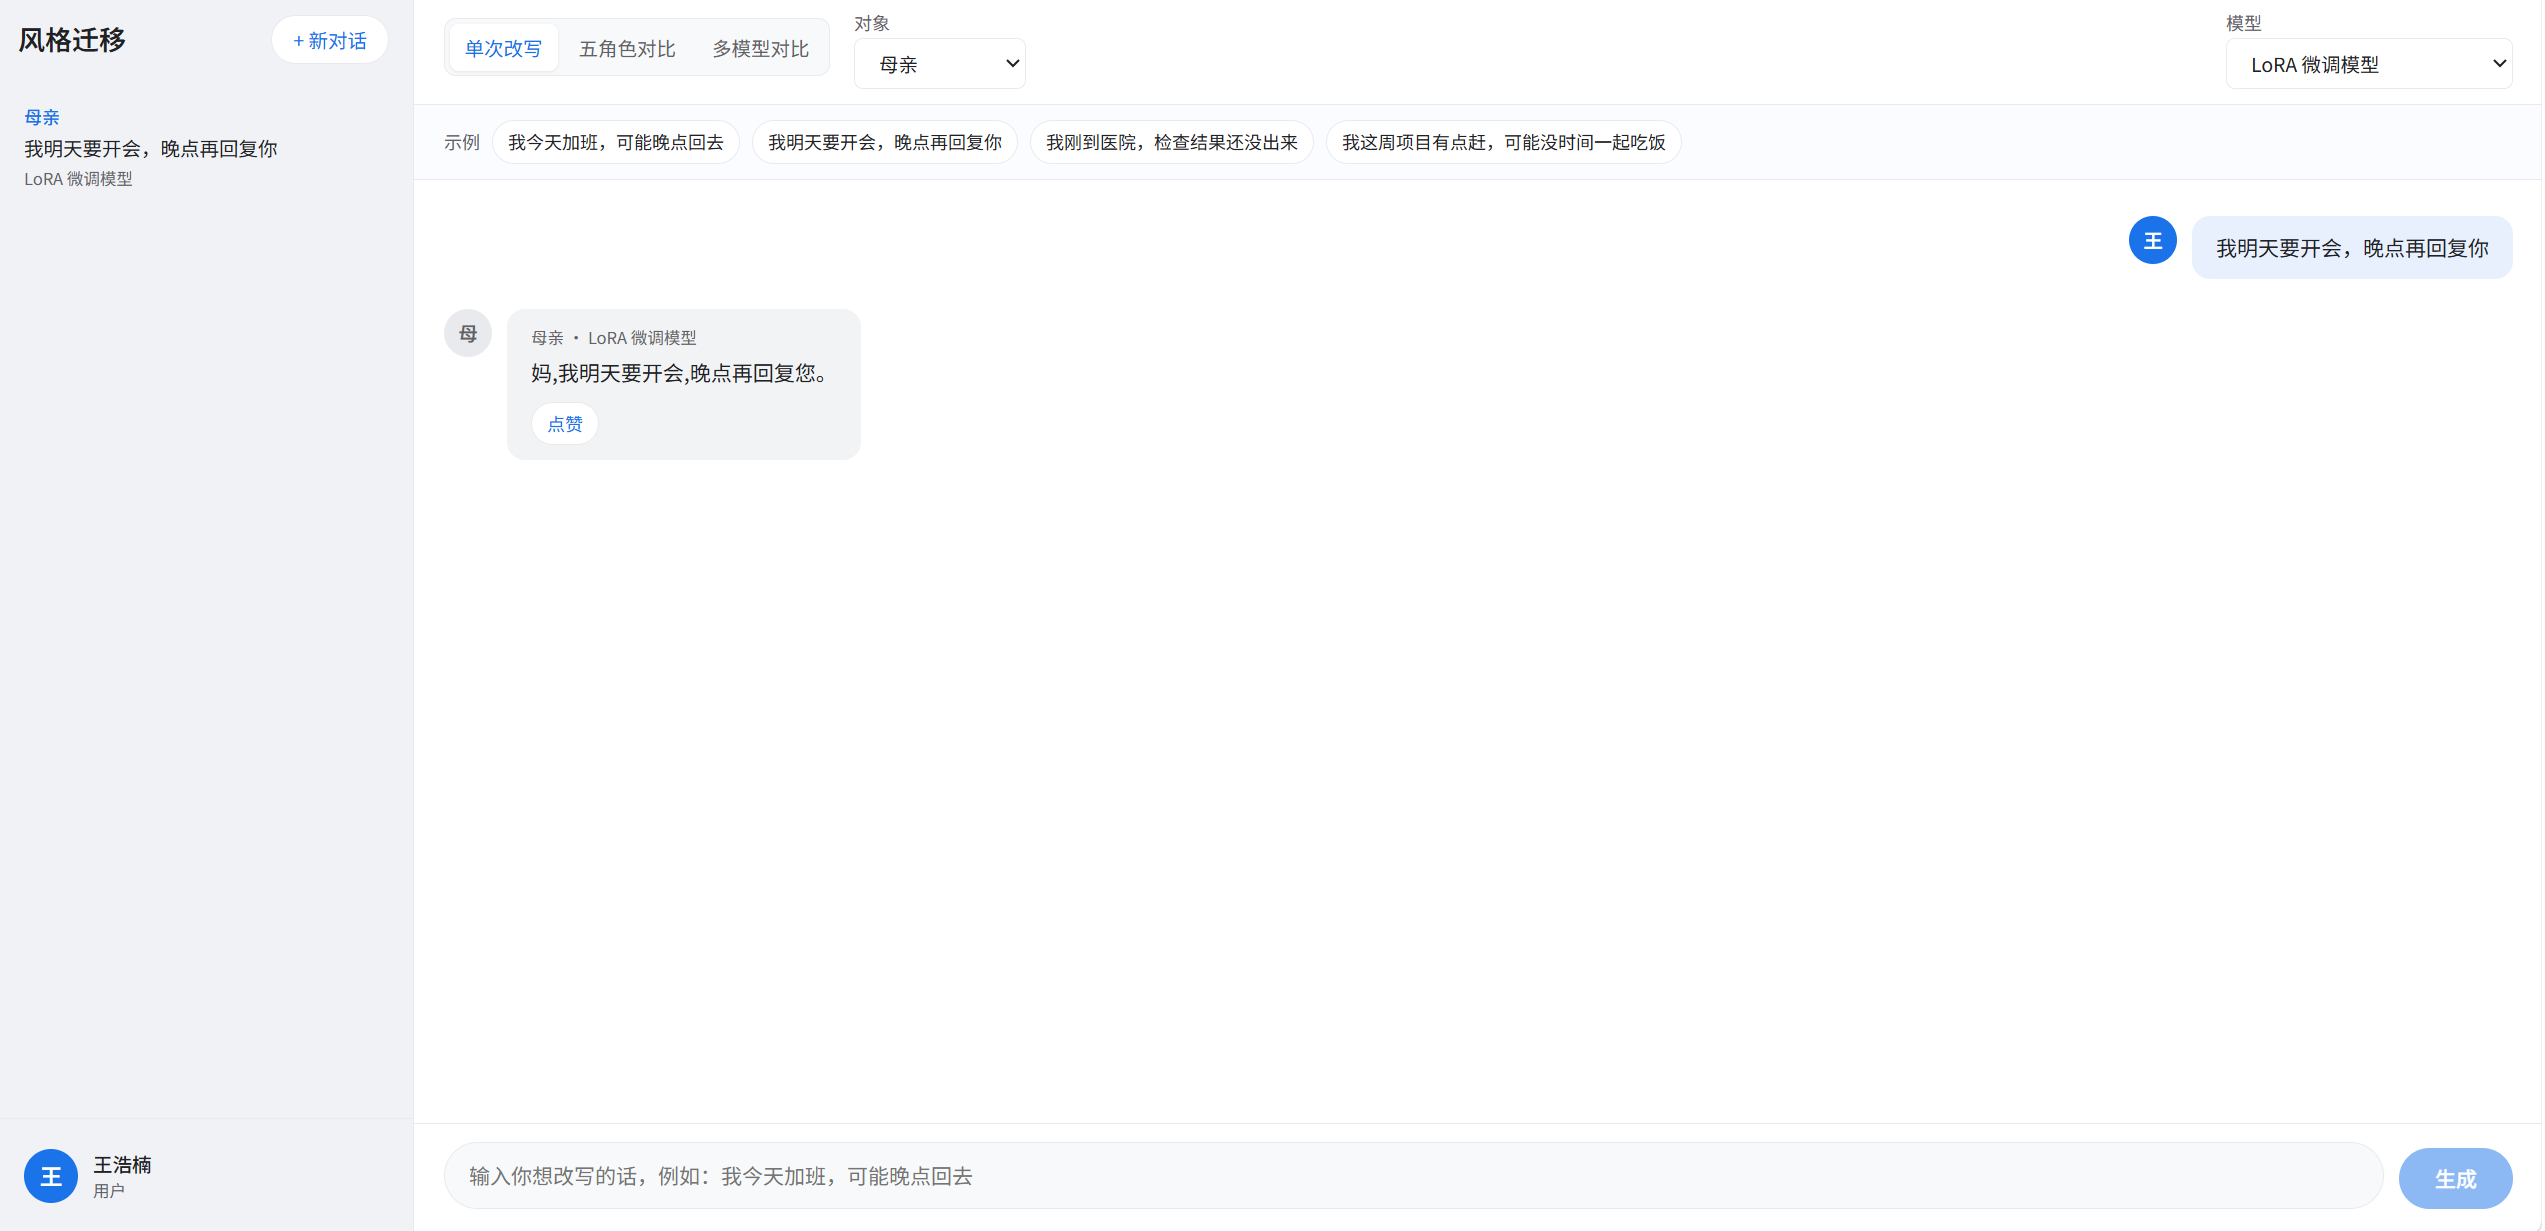
\includegraphics[width=0.9\textwidth]{figures/single_rewrite_mother_lora.png}
\caption{单次改写示例：面向母亲的 LoRA 微调模型输出}
\label{fig:single_rewrite_mother_lora}
\end{figure}

\begin{figure}[H]
\centering
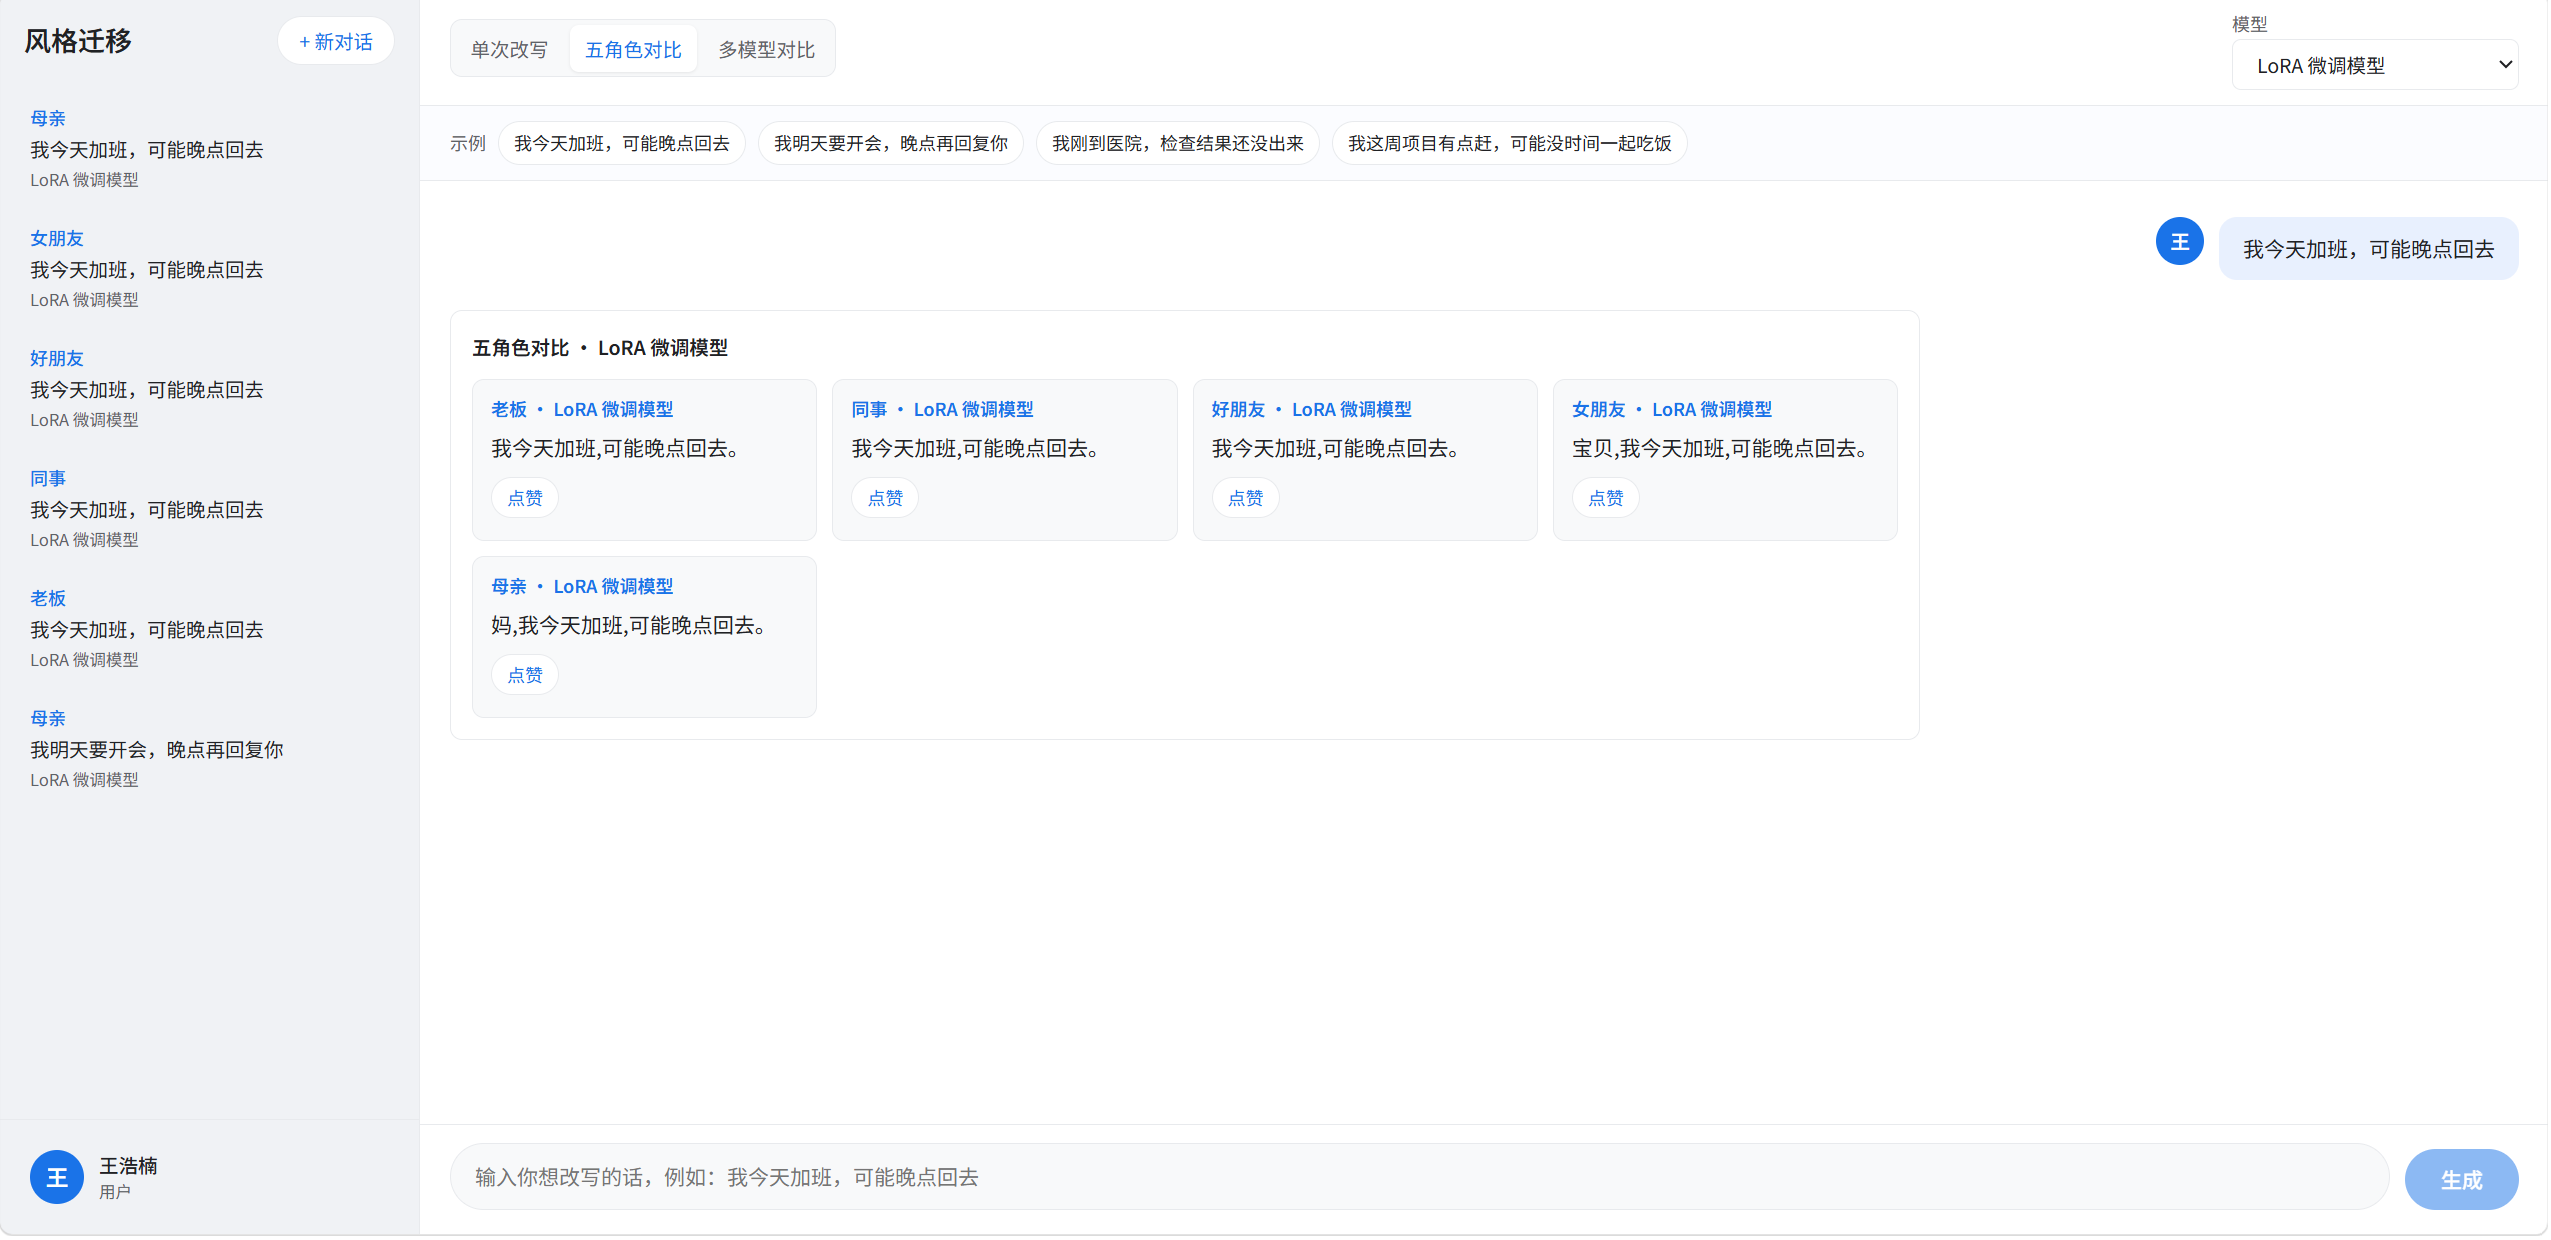
\includegraphics[width=0.9\textwidth]{figures/role_compare_lora.png}
\caption{五角色对比示例：同一句话在不同目标对象下的表达差异}
\label{fig:role_compare_lora}
\end{figure}

\begin{figure}[H]
\centering
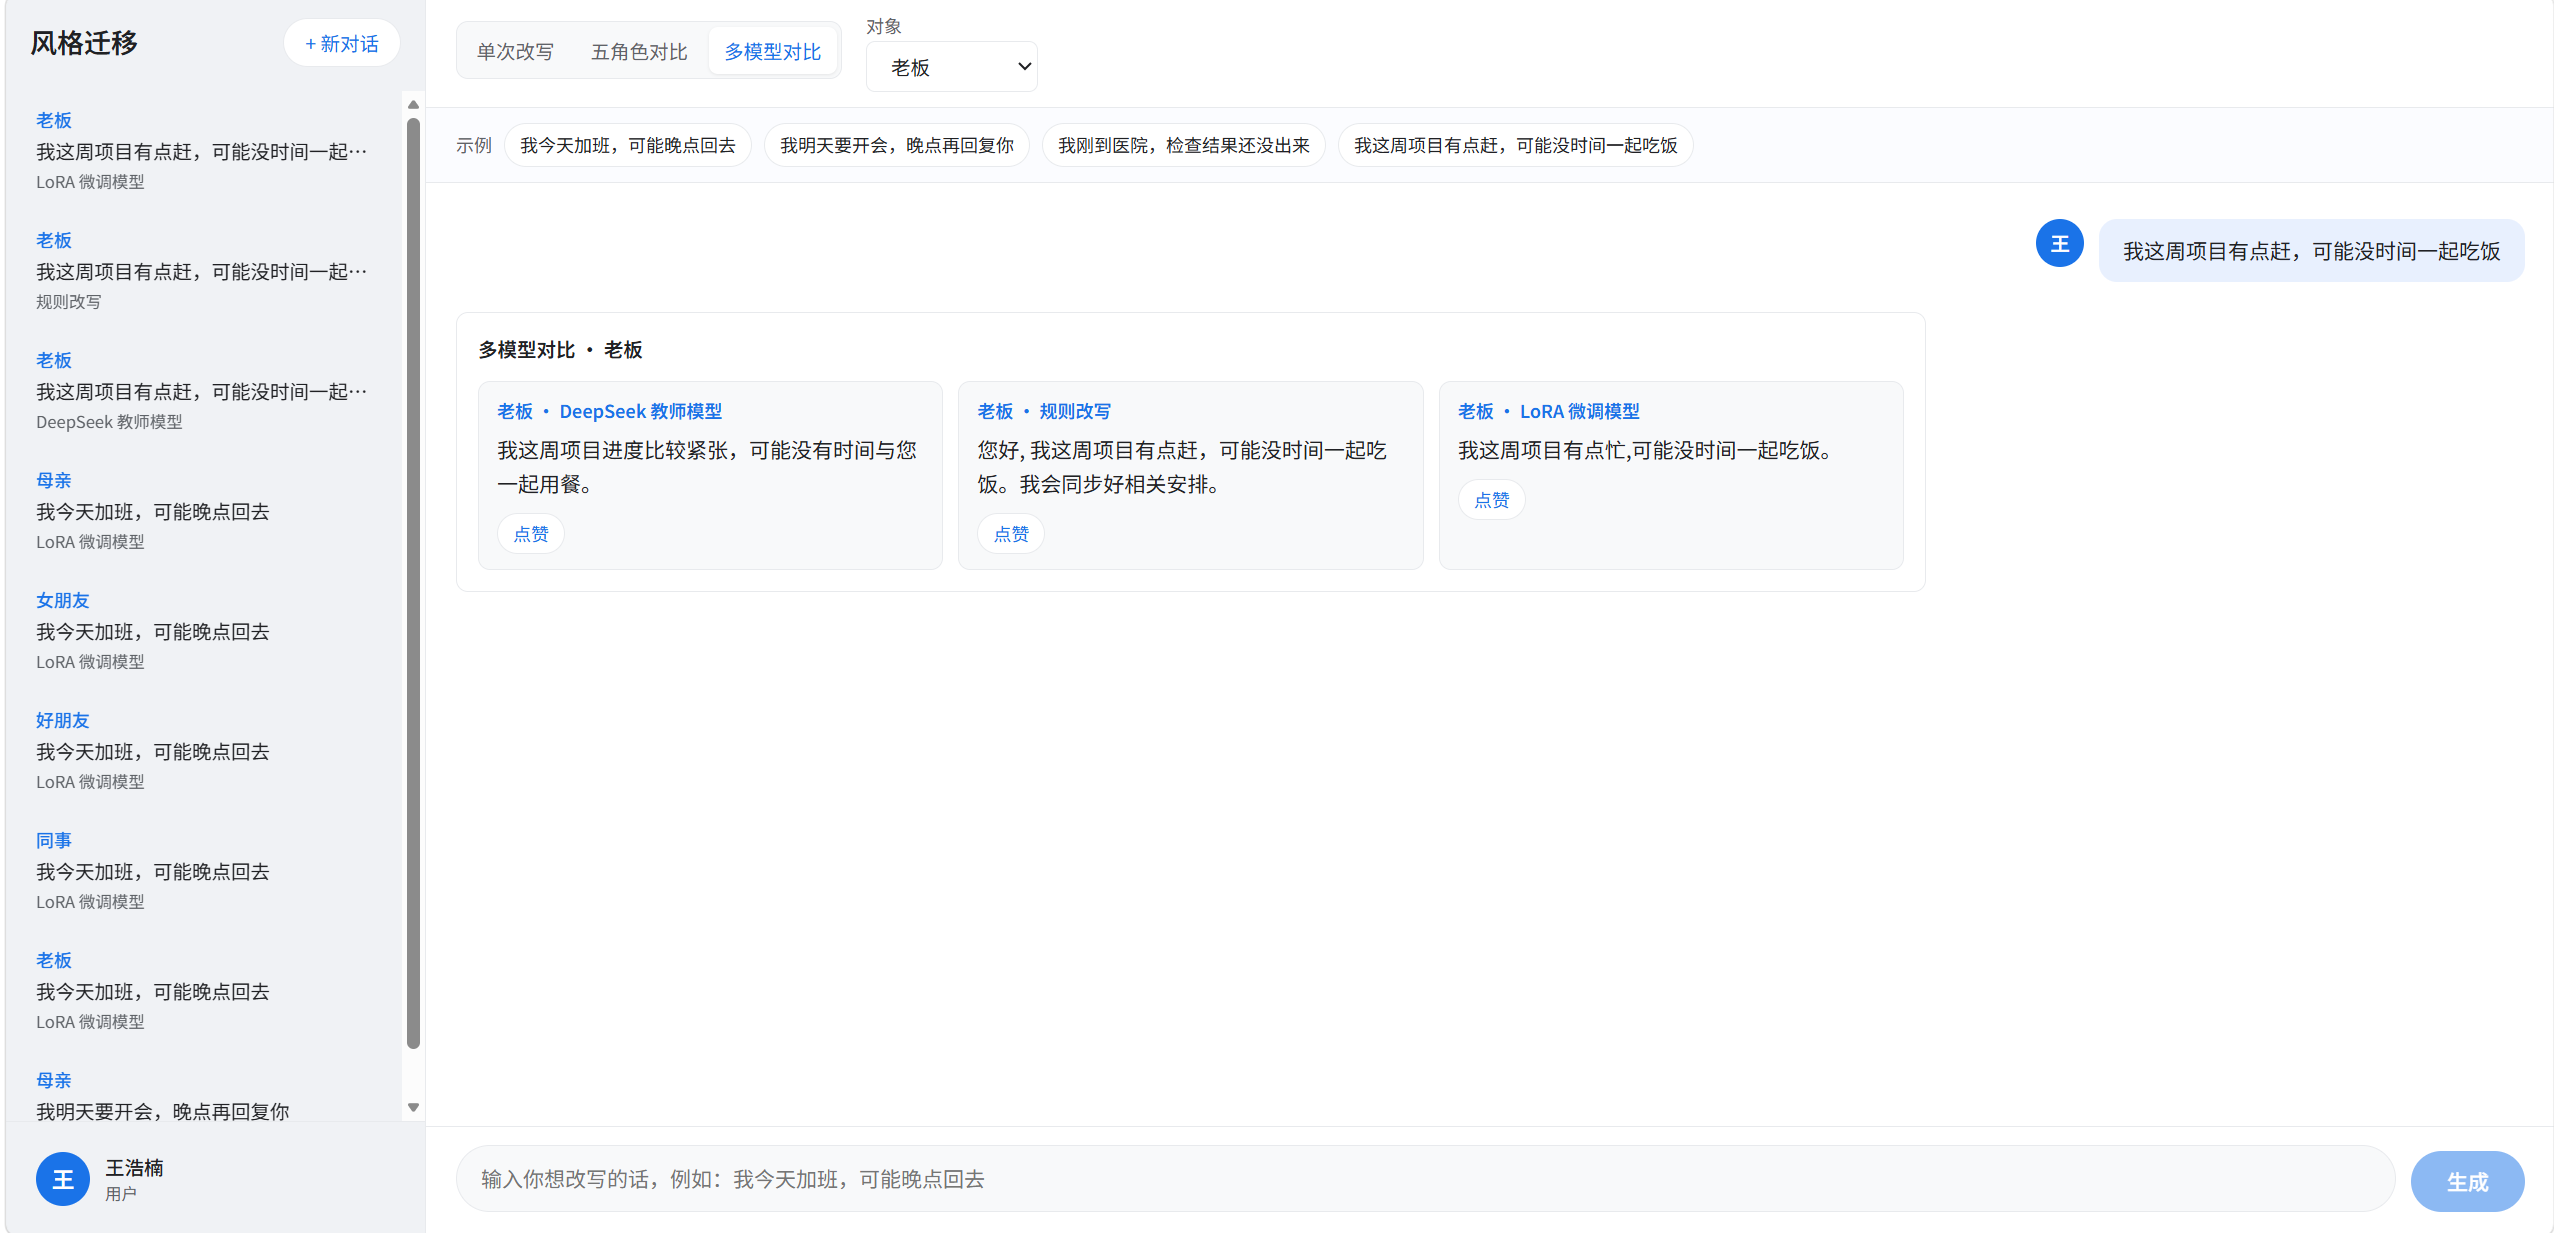
\includegraphics[width=0.9\textwidth]{figures/model_compare_boss.png}
\caption{多模型对比示例：老板对象下不同模型的输出差异}
\label{fig:model_compare_boss}
\end{figure}

图~\ref{fig:single_rewrite_mother_lora} 展示了单次改写流程，使用 LoRA 微调模型将输入句子改写为更适合对母亲表达的语气。图~\ref{fig:role_compare_lora} 展示了五角色对比功能，同一原句在老板、同事、好朋友、女朋友和母亲五类对象下生成不同表达。图~\ref{fig:model_compare_boss} 展示了多模型对比功能，可用于观察 DeepSeek 教师模型、规则改写 baseline 和 LoRA 微调模型之间的差异。

\begin{figure}[H]
\centering

\includegraphics[width=0.75\textwidth]{figures/liked_result.png}
\caption{用户点赞反馈状态}
\label{fig:liked_result}
\end{figure}

系统将原先的“采纳”行为调整为用户侧“点赞”反馈。用户认为某条改写结果较好时可以点赞，点赞结果不会直接进入训练集，而是进入管理员待审核样本池。

\begin{figure}[H]
\centering
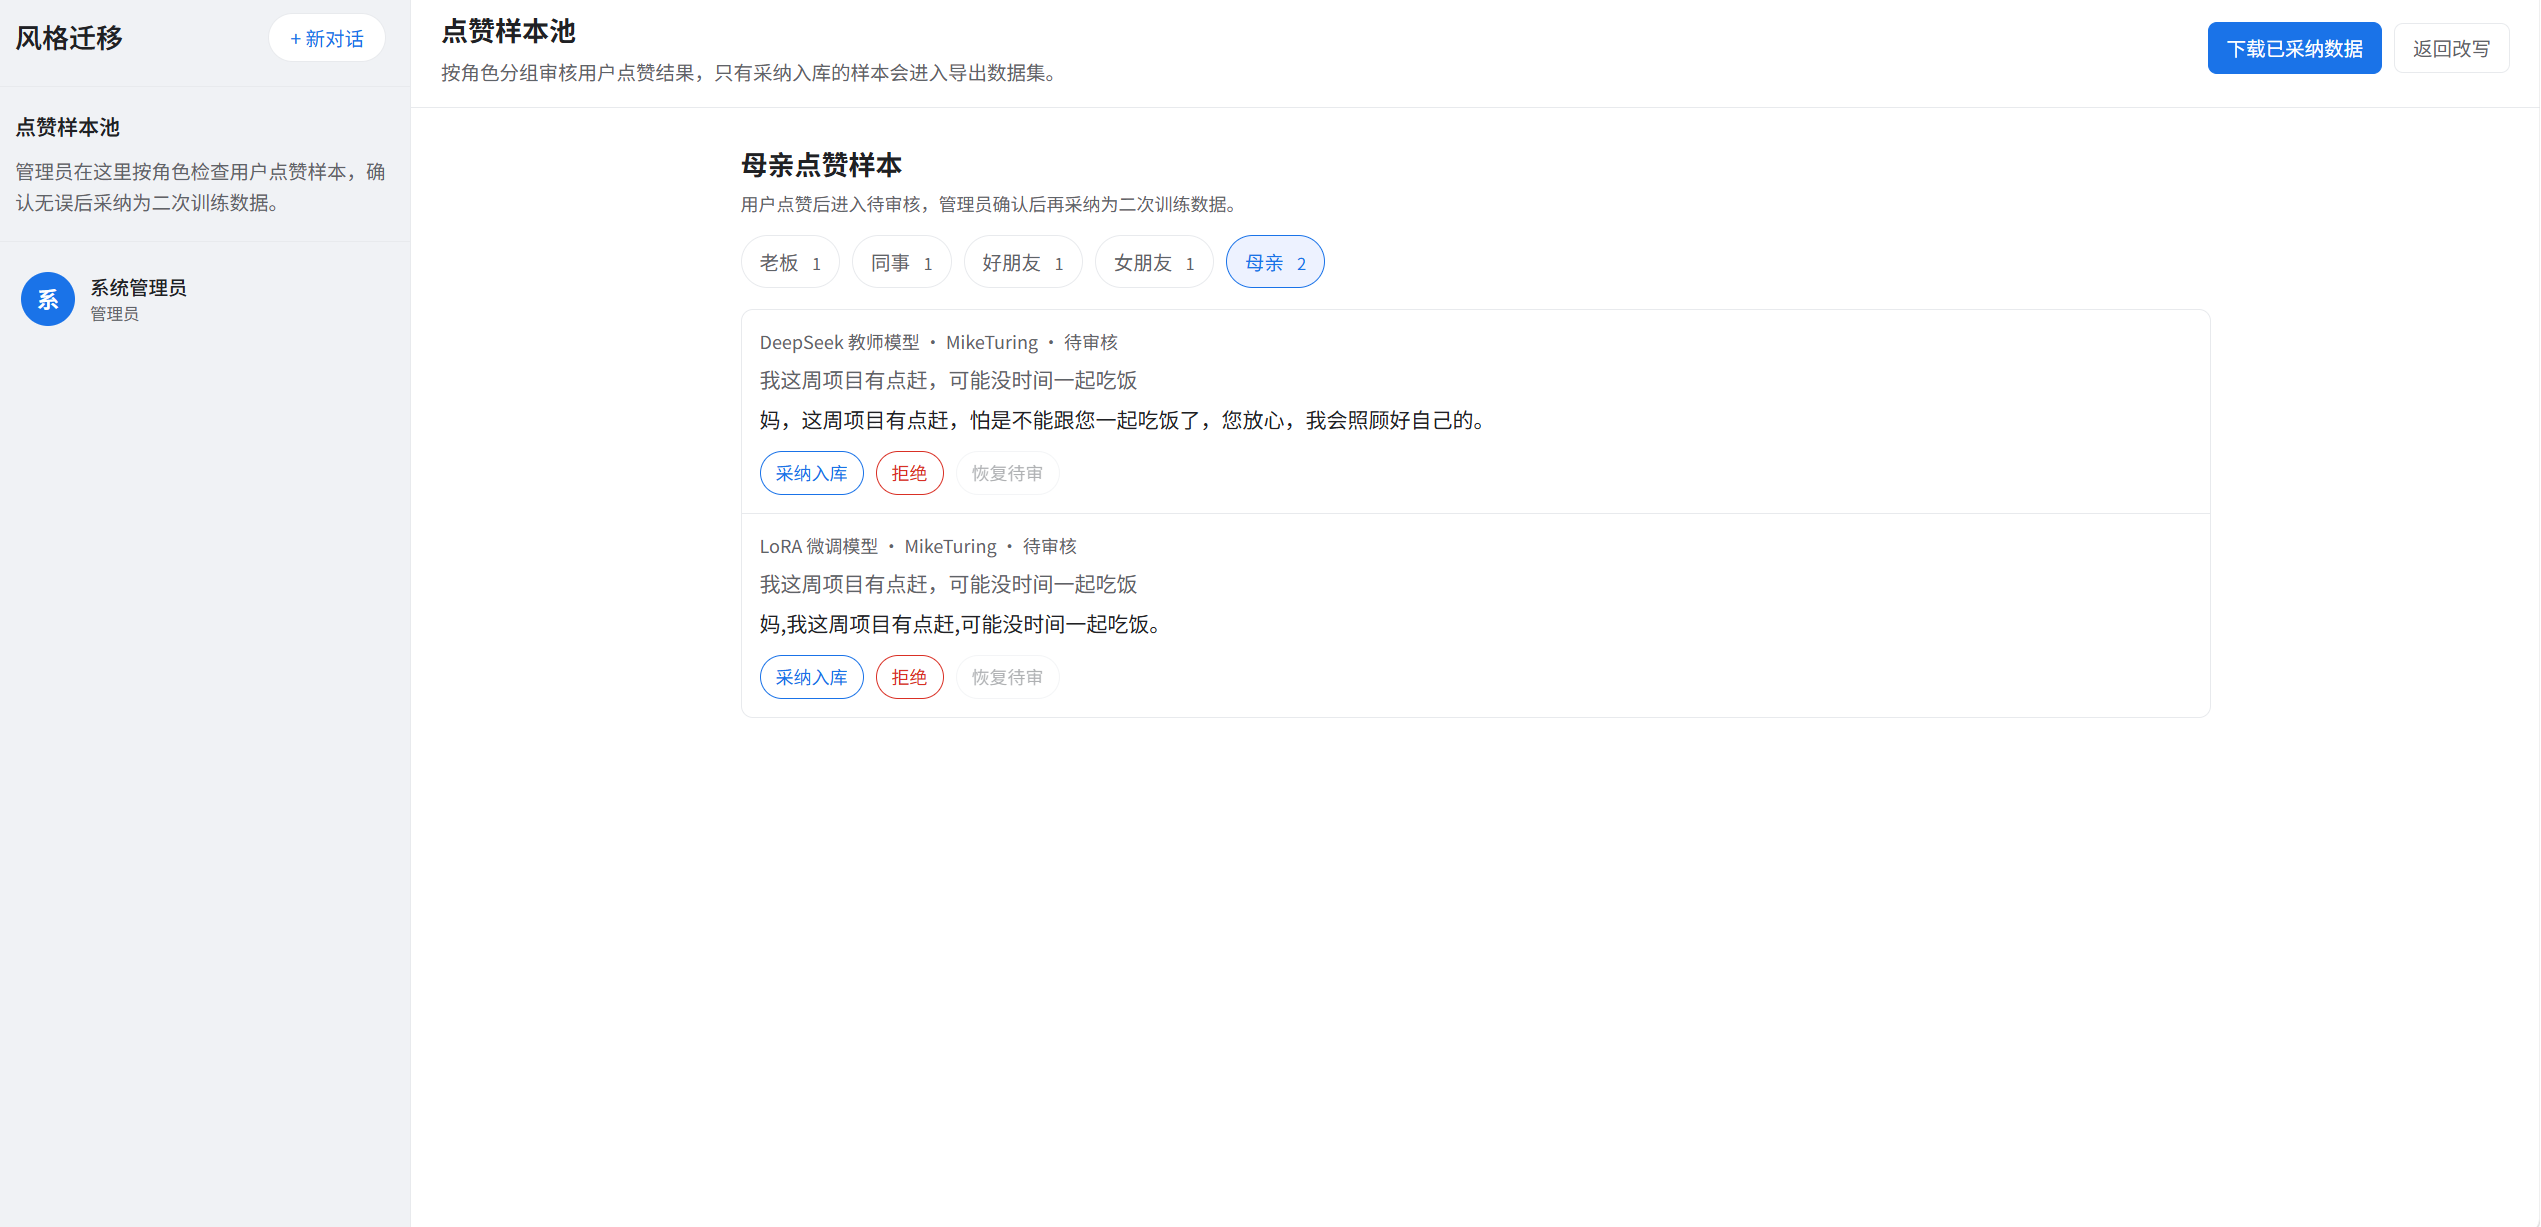
\includegraphics[width=0.9\textwidth]{figures/admin_sample_pool_grouped.png}
\caption{管理员点赞样本池：按角色选项卡查看样本}
\label{fig:admin_sample_pool_grouped}
\end{figure}

\begin{figure}[H]
\centering
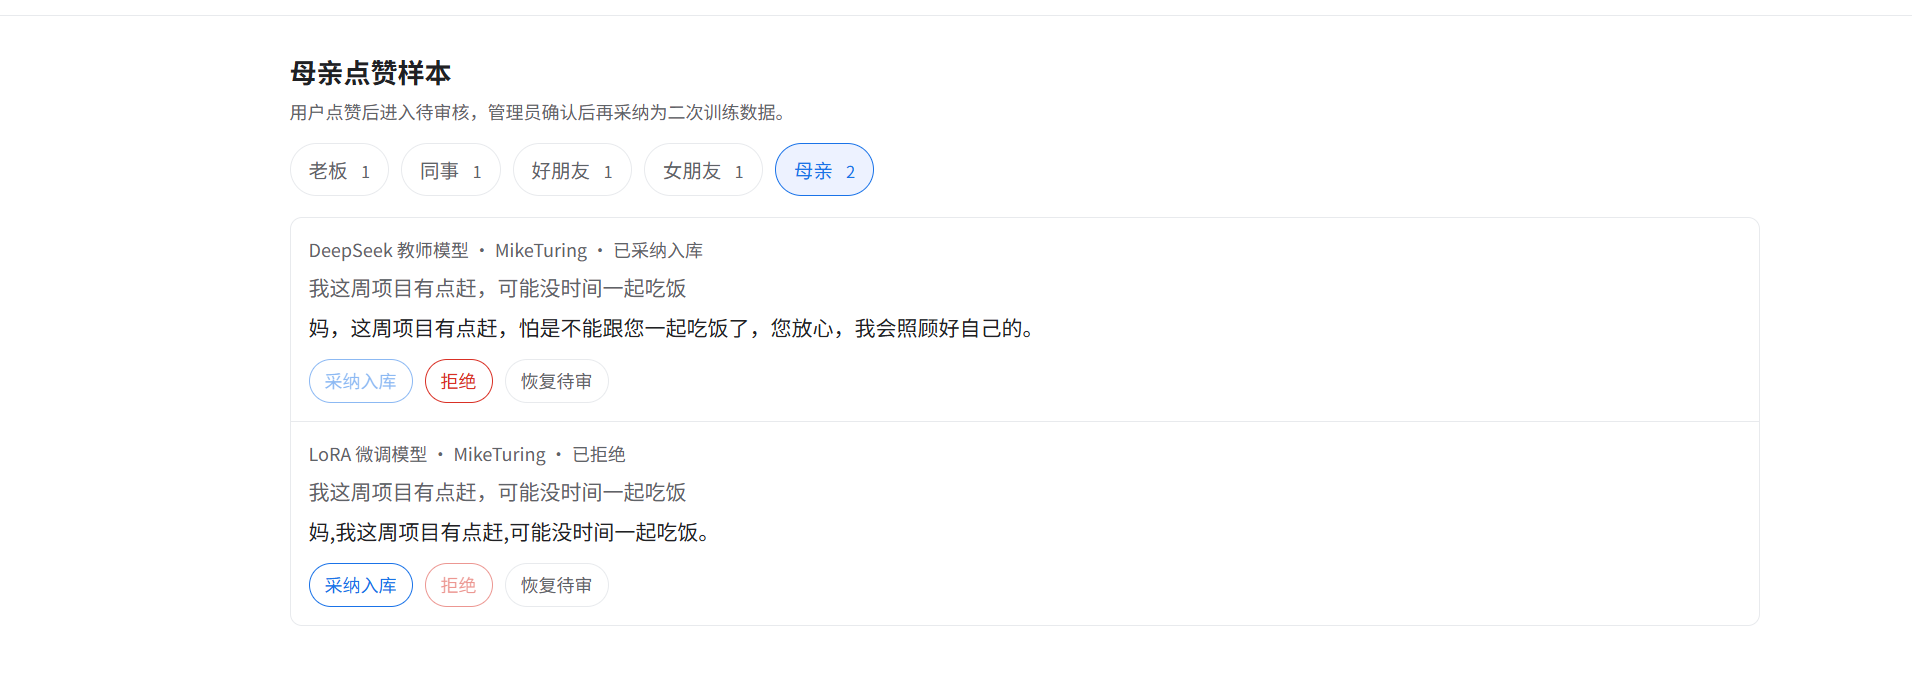
\includegraphics[width=0.9\textwidth]{figures/sample_review_actions.png}
\caption{管理员样本审核操作}
\label{fig:sample_review_actions}
\end{figure}

图~\ref{fig:admin_sample_pool_grouped} 展示了管理员端点赞样本池。系统按照目标角色设置选项卡，管理员可分别查看不同角色下的用户点赞样本，降低样本混杂带来的审核成本。图~\ref{fig:sample_review_actions} 展示了二次审核流程，管理员可将样本标记为“采纳入库”“拒绝”或“恢复待审”。只有审核通过的样本才会作为后续二次训练数据。

\begin{figure}[H]
\centering
\begin{minipage}{0.48\textwidth}
\centering
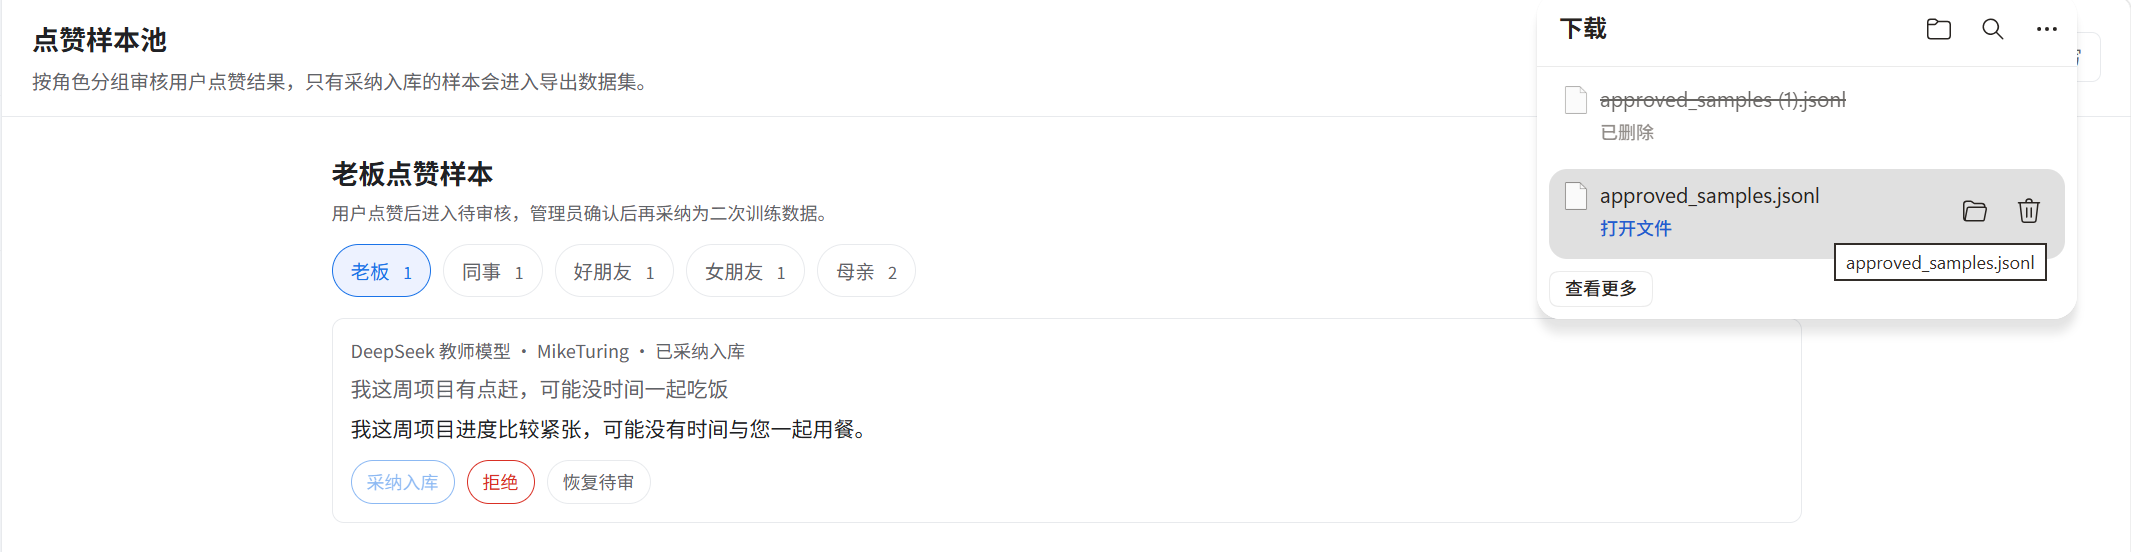
\includegraphics[width=\textwidth]{figures/export_approved_samples1.png}
\caption{已采纳样本下载入口}
\label{fig:export_approved_samples1}
\end{minipage}
\hfill
\begin{minipage}{0.48\textwidth}
\centering
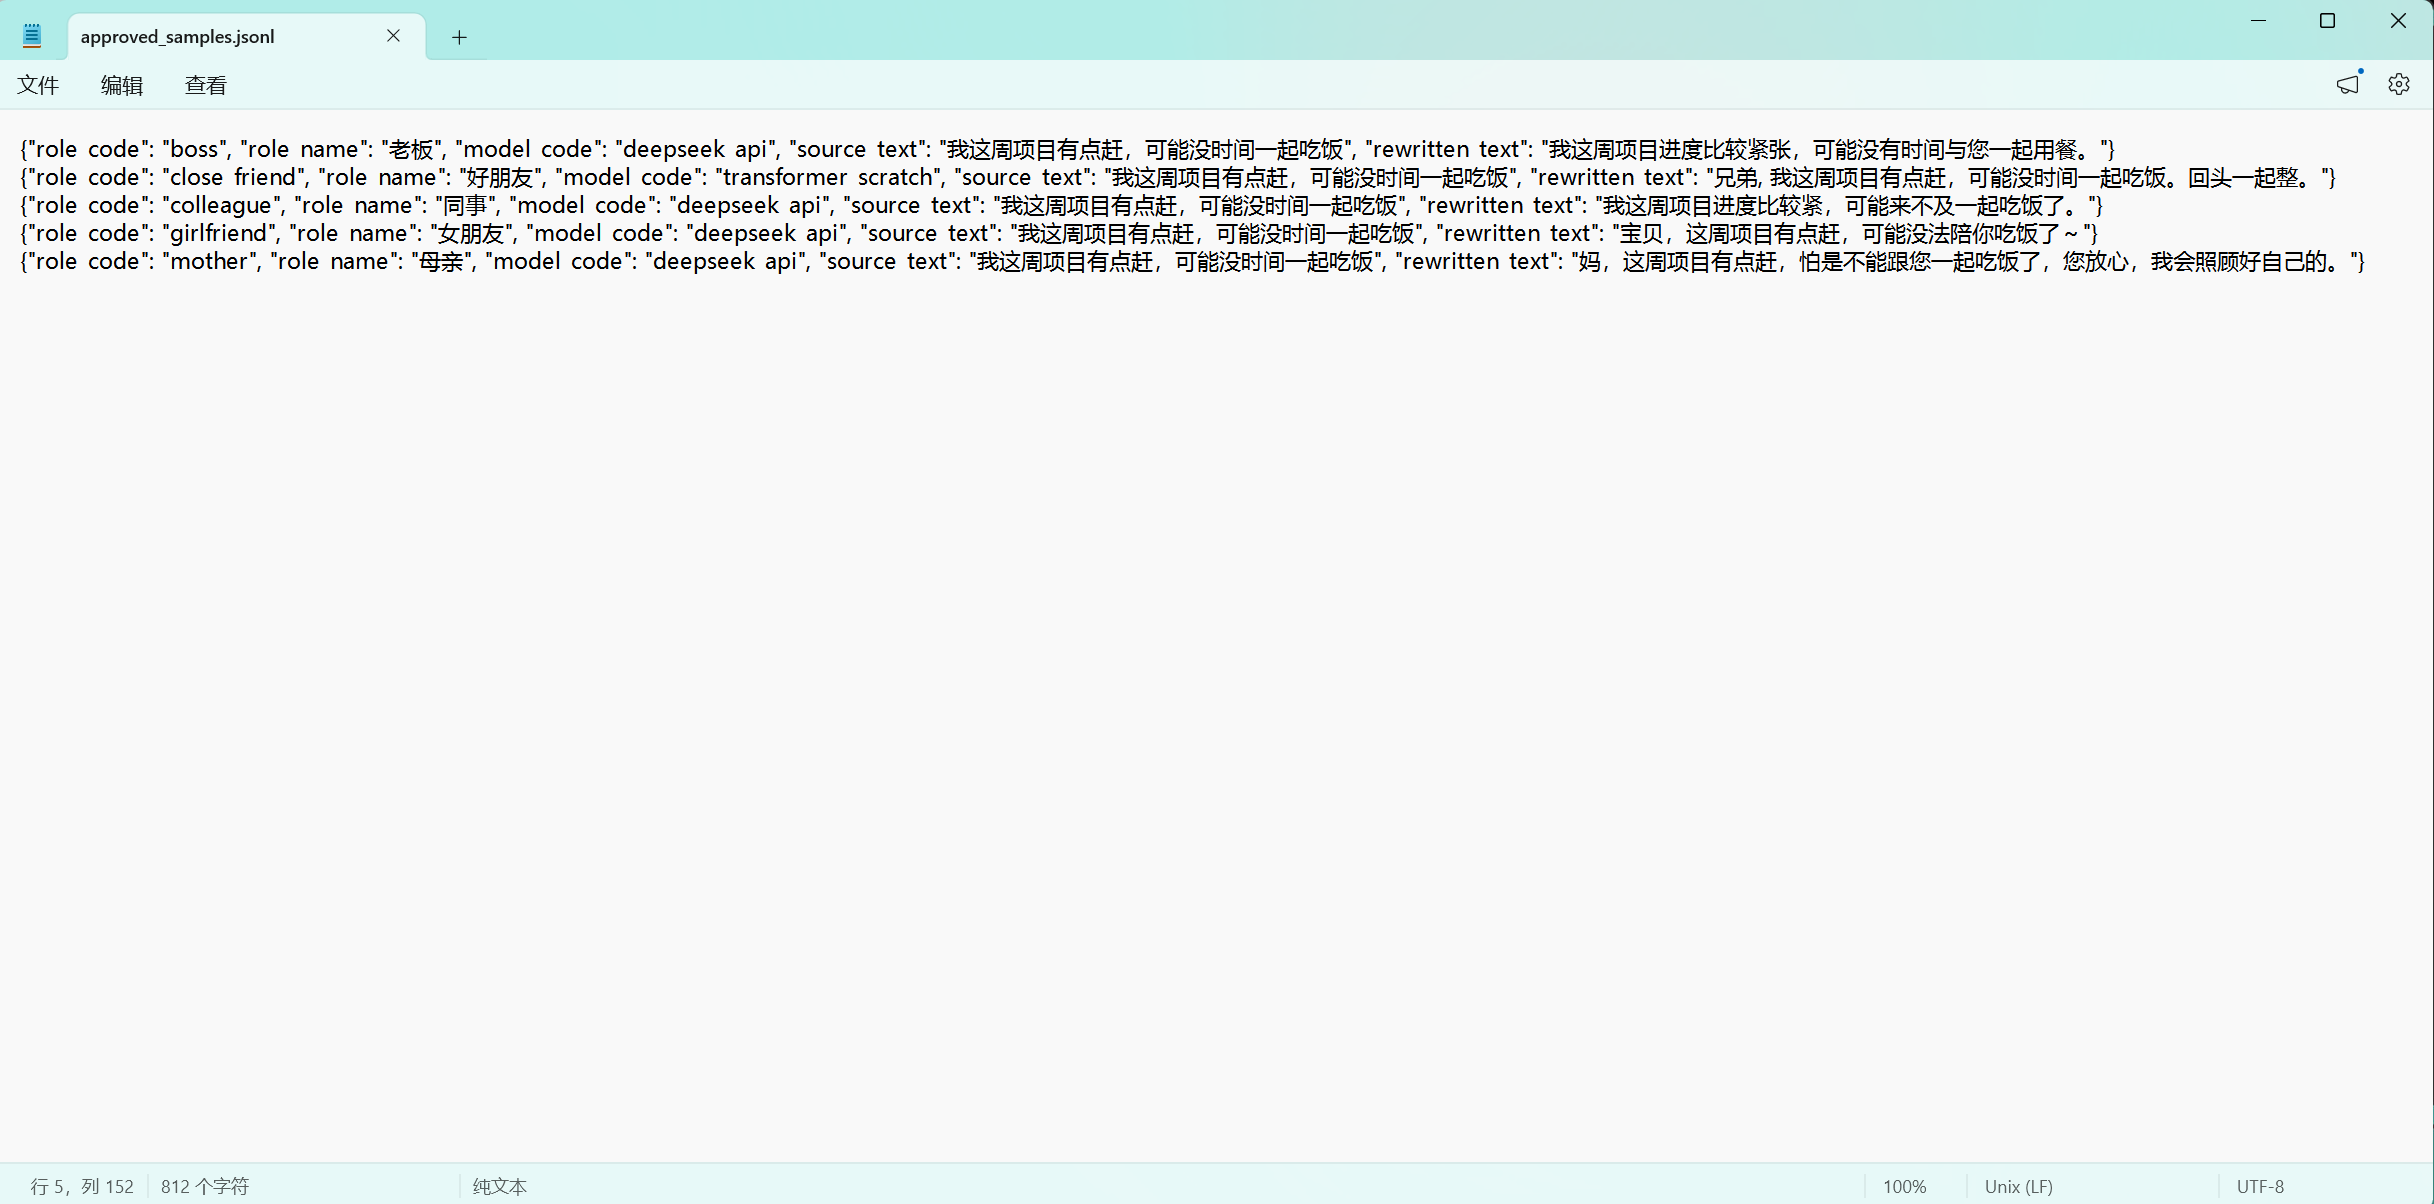
\includegraphics[width=\textwidth]{figures/export_approved_samples2.png}
\caption{已采纳样本导出结果}
\label{fig:export_approved_samples2}
\end{minipage}
\end{figure}

图~\ref{fig:export_approved_samples1} 和图~\ref{fig:export_approved_samples2} 展示了已采纳样本的导出功能。管理员可将审核通过的样本下载为本地数据文件，便于与原训练集拼接后继续进行 LoRA 增量训练。

\begin{figure}[H]
\centering

\includegraphics[height=0.6\textheight]{figures/history_records.png}
\caption{历史记录展示}
\label{fig:history_records}
\end{figure}

图~\ref{fig:history_records} 展示了系统历史记录功能。用户可以回看先前输入、目标角色、模型类型和改写结果，从而支持结果复查和样本追踪。

\subsubsection{华为云部署与运行验证}

为满足项目在云端可运行、可访问、可演示的要求，本项目将前端、后端和数据库部署到华为云弹性云服务器。服务器公网 IP 为 \texttt{119.3.170.13}，前端通过 \texttt{5173} 端口对外提供访问，后端 FastAPI 服务通过 \texttt{8000} 端口提供接口。部署验证过程不仅关注页面是否能打开，还需要确认代码已在云服务器中启动、模型服务已加载、接口请求能够返回正常状态，并且浏览器端能够通过公网 IP 完成系统访问。

\begin{figure}[H]
\centering
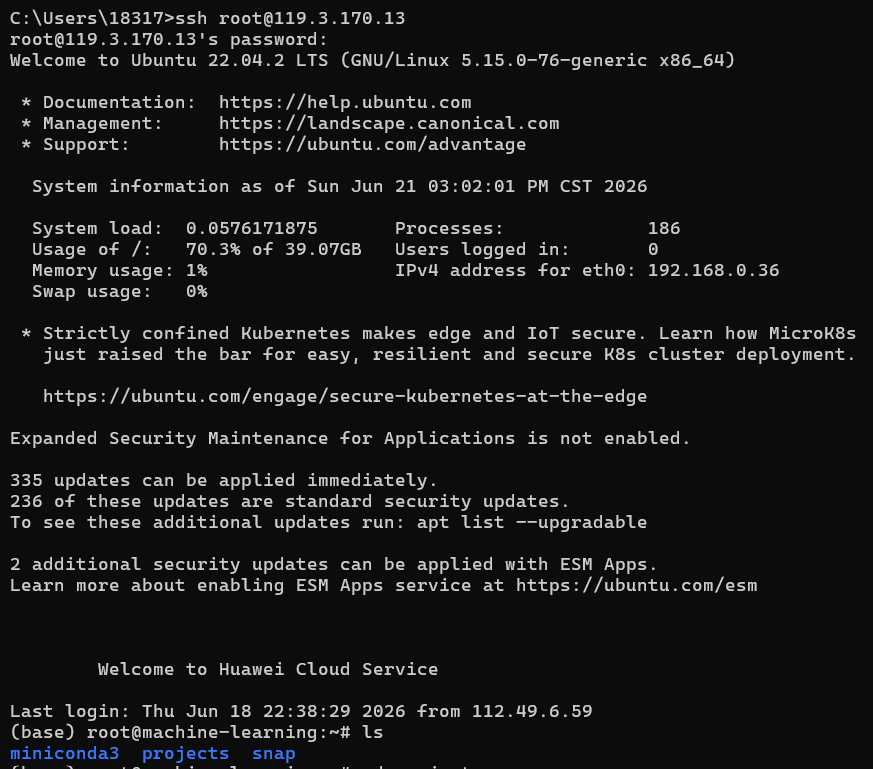
\includegraphics[width=0.9\textwidth]{figures/huawei_ssh_login.png}
\caption{通过 SSH 登录华为云服务器}
\label{fig:huawei_ssh_login}
\end{figure}

图~\ref{fig:huawei_ssh_login} 展示了通过 \texttt{ssh root@119.3.170.13} 登录服务器的过程。终端中出现 Ubuntu 系统信息和 Huawei Cloud Service 提示，说明当前操作环境为华为云服务器，而不是本地开发环境。

\begin{figure}[H]
\centering
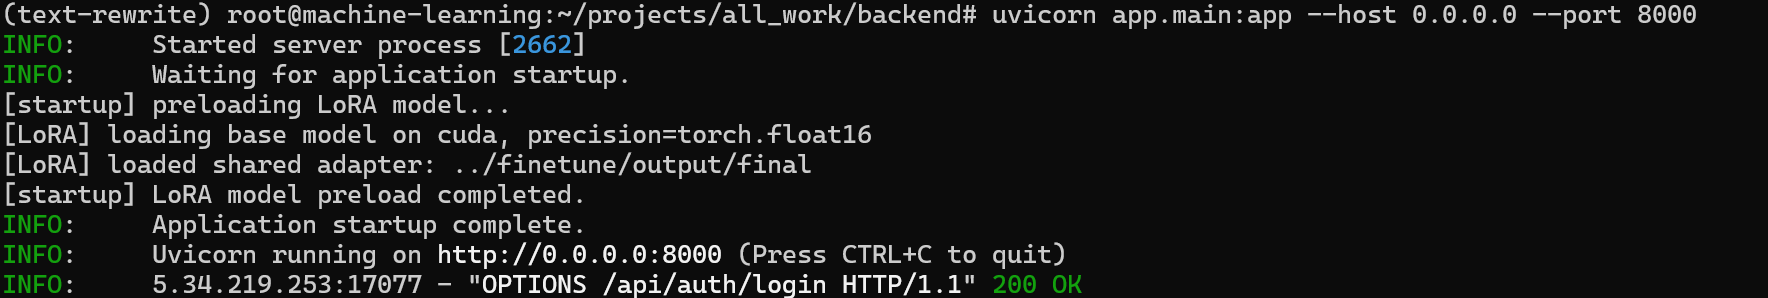
\includegraphics[width=0.95\textwidth]{figures/huawei_backend_start.png}
\caption{华为云服务器后端服务启动结果}
\label{fig:huawei_backend_start}
\end{figure}

图~\ref{fig:huawei_backend_start} 展示了后端服务在服务器中的启动过程。项目进入 \texttt{backend} 目录后执行 \texttt{uvicorn app.main:app --host 0.0.0.0 --port 8000}，服务启动时会预加载 LoRA 模型，并显示 \texttt{Uvicorn running on http://0.0.0.0:8000}。日志中还出现登录接口的 \texttt{200 OK} 返回，说明后端接口已能够接收来自前端的请求。

\begin{figure}[H]
\centering
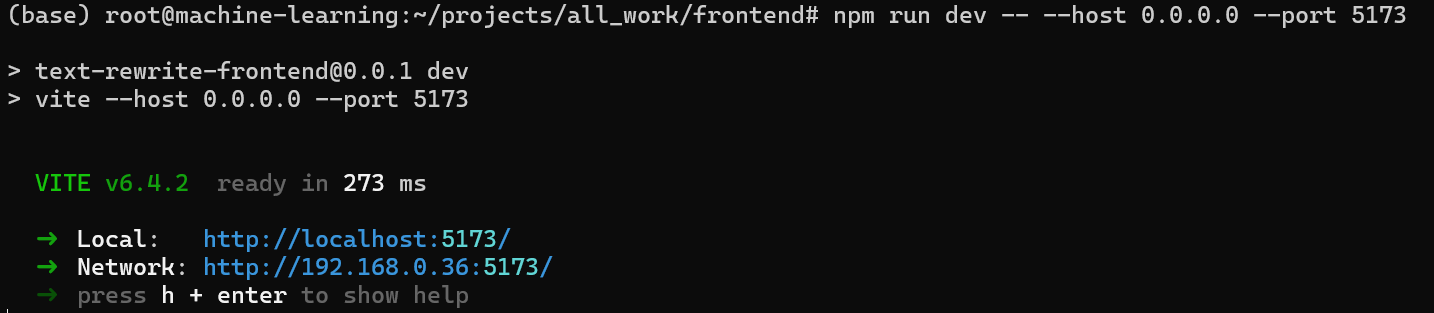
\includegraphics[width=0.95\textwidth]{figures/huawei_frontend_start.png}
\caption{华为云服务器前端服务启动结果}
\label{fig:huawei_frontend_start}
\end{figure}

图~\ref{fig:huawei_frontend_start} 展示了前端服务在服务器中的启动过程。项目进入 \texttt{frontend} 目录后执行 \texttt{npm run dev -- --host 0.0.0.0 --port 5173}，Vite 服务成功启动，并绑定到 \texttt{0.0.0.0}。该设置使前端页面不仅能在服务器本地访问，也能通过公网 IP 和端口被外部浏览器访问。

\begin{figure}[H]
\centering
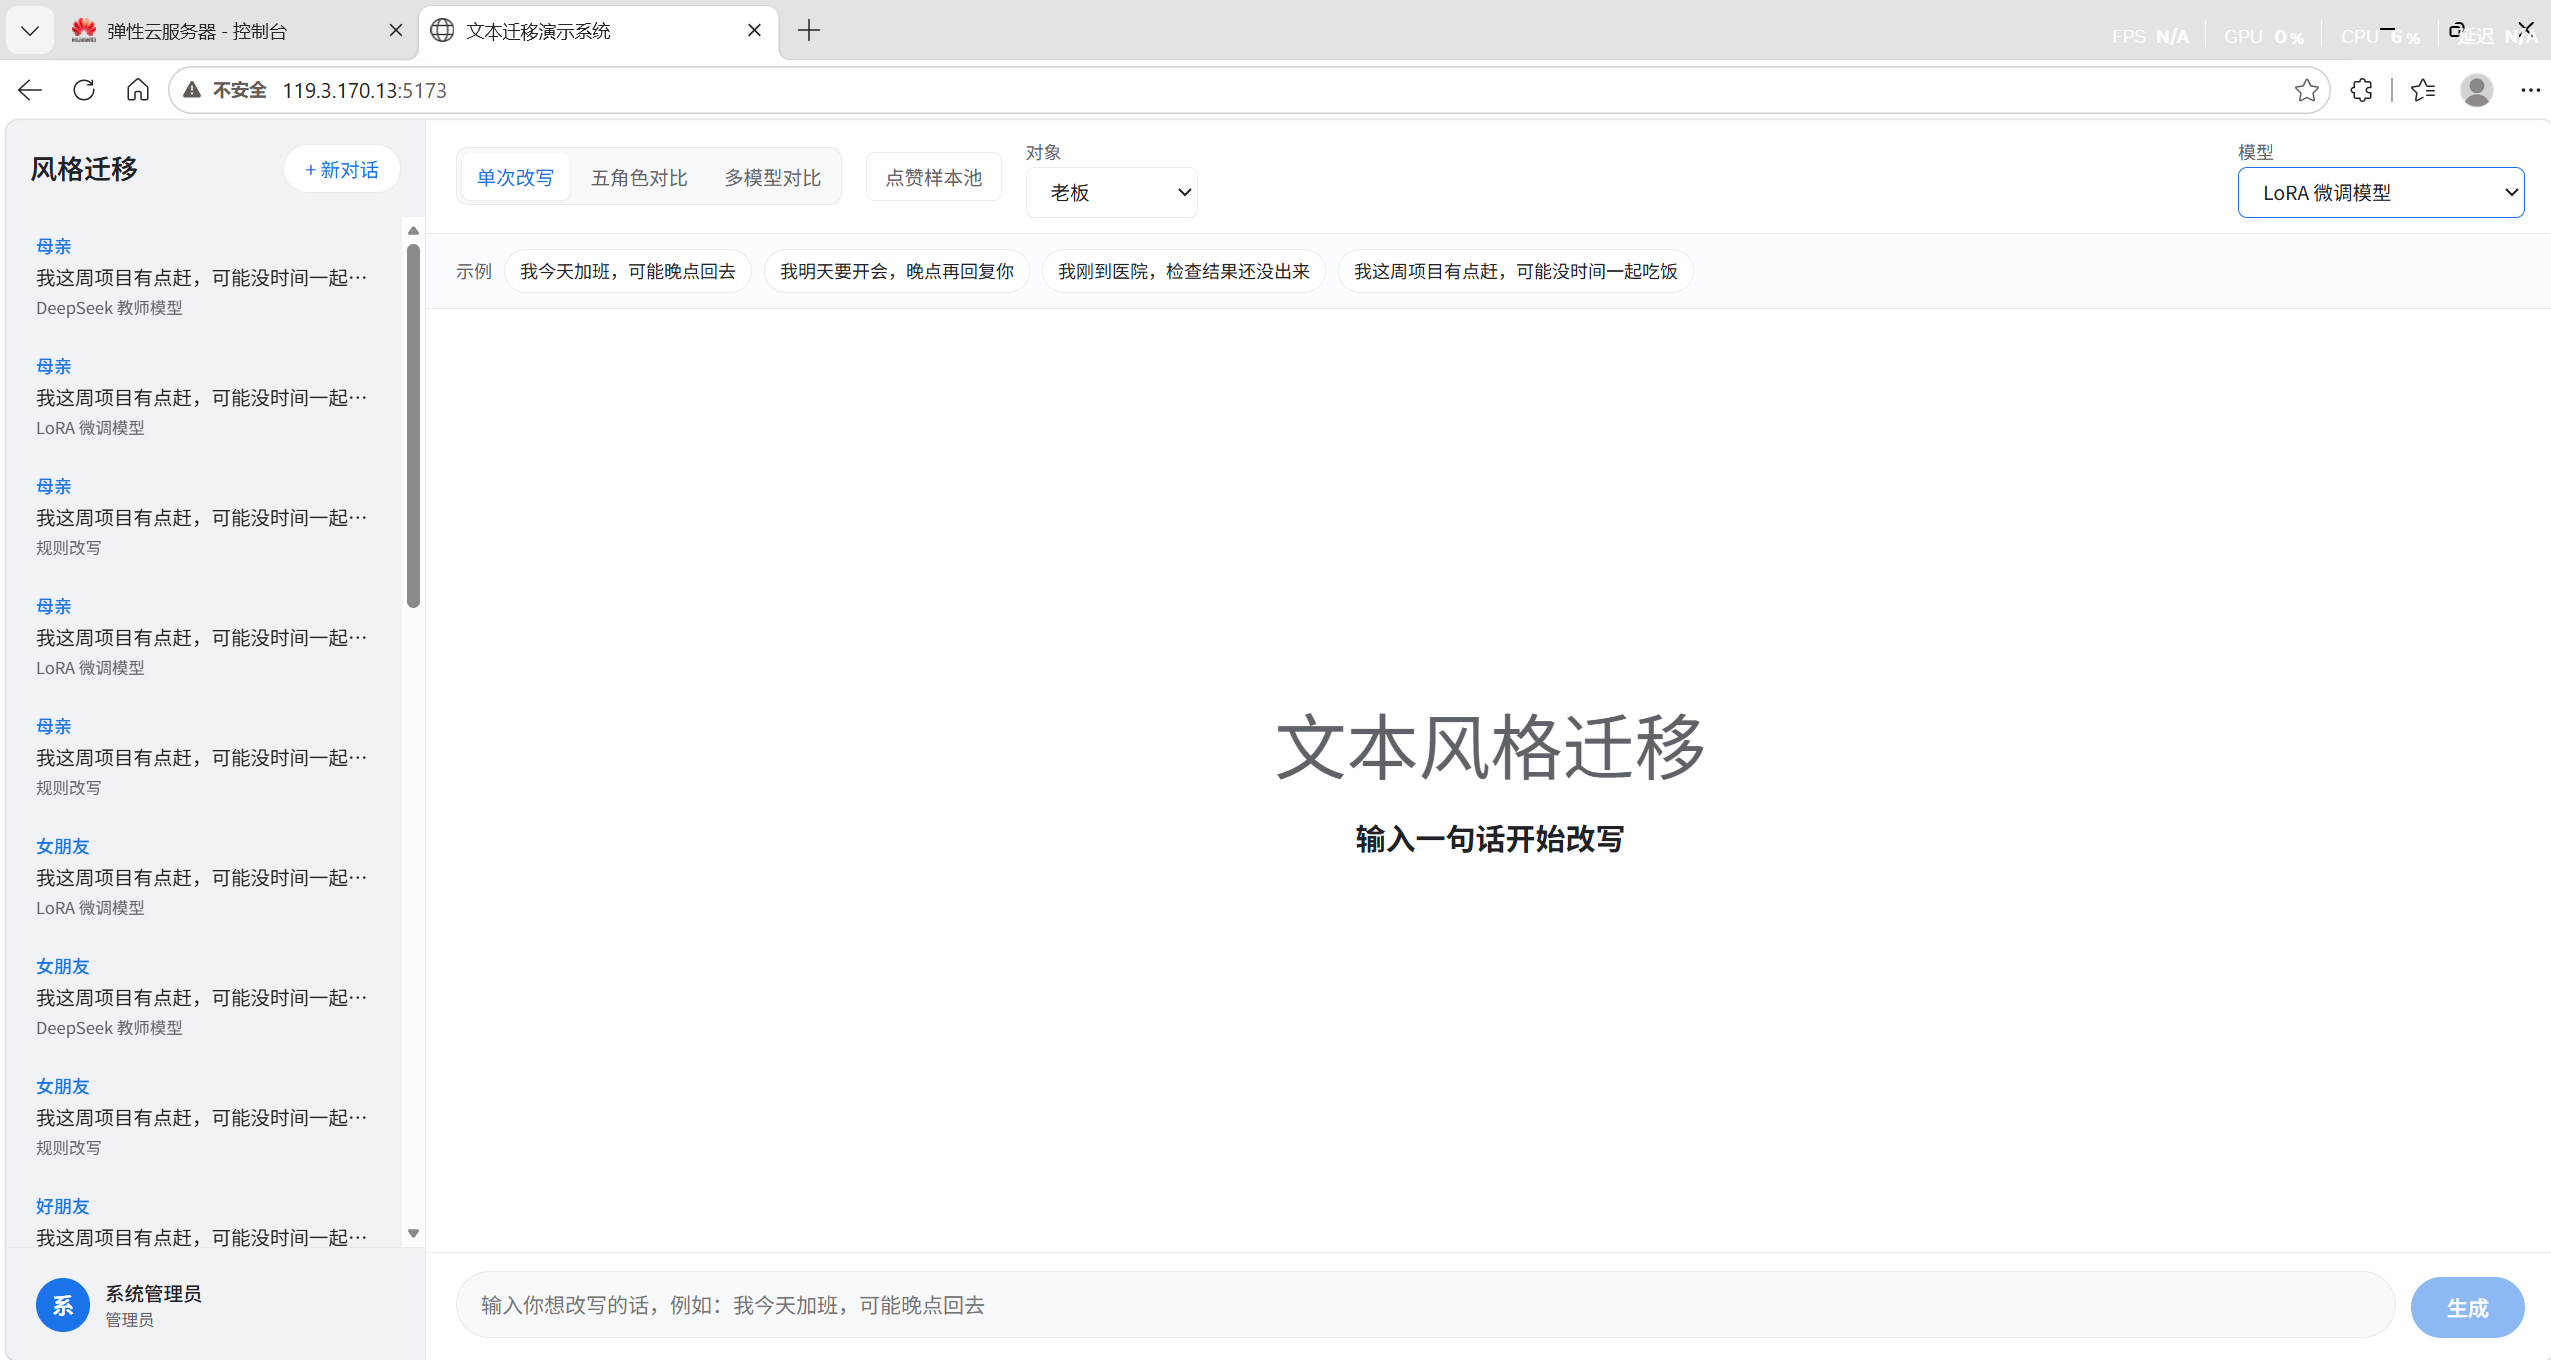
\includegraphics[width=\textwidth]{figures/huawei_public_ip_access.png}
\caption{通过公网 IP 和端口访问前端系统}
\label{fig:huawei_public_ip_access}
\end{figure}

图~\ref{fig:huawei_public_ip_access} 展示了浏览器通过 \texttt{http://119.3.170.13:5173} 访问系统的结果。页面标题、角色选择、模型选择、历史记录和输入框均能正常显示，说明前端页面已经从云服务器对外提供服务。结合后端启动日志中的接口返回结果，可以证明系统已经完成前端、后端、模型推理服务与数据库的云端联调。

\begin{figure}[H]
\centering
\begin{minipage}{0.48\textwidth}
\centering
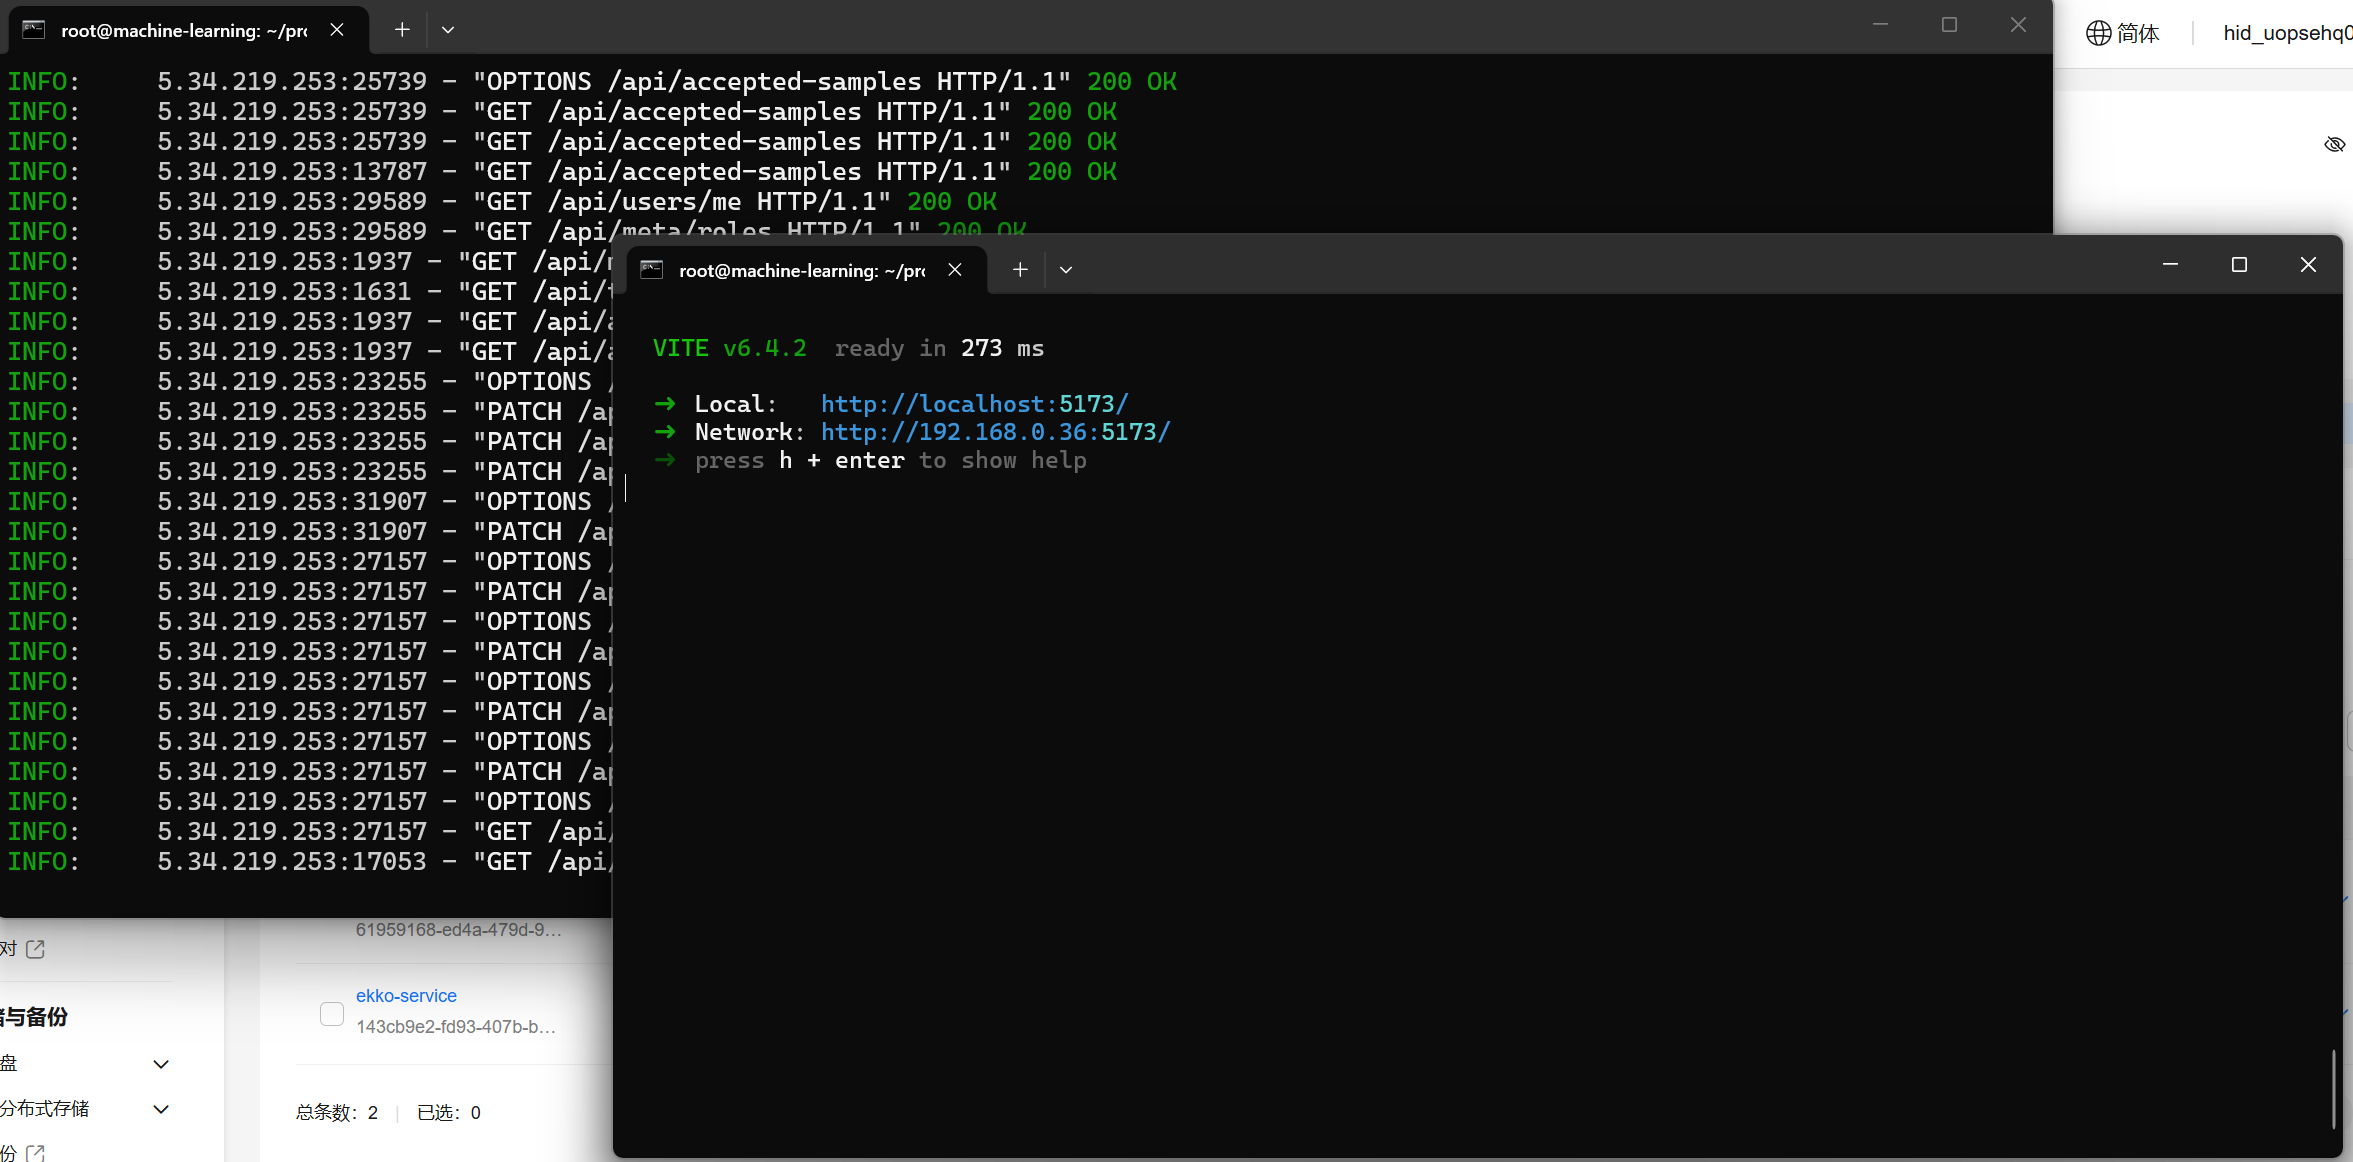
\includegraphics[width=\textwidth]{figures/server_deployment.png}
\caption{服务器公网访问效果}
\label{fig:server_deployment}
\end{minipage}
\hfill
\begin{minipage}{0.48\textwidth}
\centering
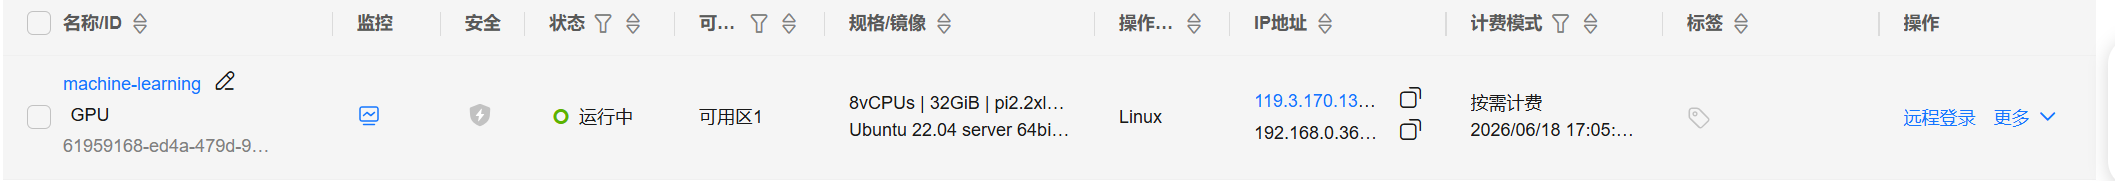
\includegraphics[width=\textwidth]{figures/server_deployment1.png}
\caption{服务器运行状态}
\label{fig:server_deployment1}
\end{minipage}
\end{figure}

图~\ref{fig:server_deployment} 和图~\ref{fig:server_deployment1} 进一步展示了项目部署后的访问和运行状态。整体来看，云端验证覆盖了 SSH 登录、后端代码运行、前端代码运行、公网访问和功能页面展示五个环节，能够较完整地证明本项目已在华为云服务器上完成部署。

\section{实验结果与分析}

\subsection{定量结果}

由于本任务缺乏公开标准测试集，项目主要使用自建测试集和规则指标进行初步评估。定量统计包括数据过滤比例、角色有效样本数、输出长度、语义相似度和角色输出差异。当前过滤后有效角色改写为 8957 条，相较原始教师数据去除了 1043 条风险较高的监督目标。

从质检报告看，主要问题来源包括模板式改写、原始 N/A、时间关键词丢失、数字丢失和语义相似度过低。这说明中文角色风格迁移不仅需要生成自然表达，还需要严格保护事实信息，不能简单追求“更像某个角色”。

模型训练完成后，在 897 条测试样本上进行评估，测试集 \texttt{eval\_loss} 为 1.2962，测试推理速度约为 99.58 samples/s。本次训练共进行 8 轮，最优验证指标对应 \path{output/checkpoint-6900}，训练结束后将最终适配器保存到 \path{finetune/output/final/}。这些结果主要用于说明微调过程已经正常收敛；由于本任务存在多种合理改写方式，loss 仍需与样例分析和错误案例分析结合使用。

\begin{table}[H]
\centering
\caption{LoRA 微调测试结果}
\label{tab:lora_test_metrics}
\begin{tabular}{c|c}
\toprule
指标 & 数值 \\
\midrule
测试样本数 & 897 \\
测试集 \texttt{eval\_loss} & 1.2962 \\
测试耗时 & 9.01 s \\
测试吞吐 & 99.58 samples/s \\
最佳 checkpoint & \path{output/checkpoint-6900} \\
最佳验证 loss & 1.3211 \\
\bottomrule
\end{tabular}
\end{table}

\subsection{损失指标说明}

需要说明的是，生成任务中的 loss 并不能直接等同于最终生成质量。本文任务属于开放式中文文本改写，同一原句在同一目标对象下可能存在多种合理表达方式，而训练损失主要衡量模型生成参考文本时的 token 级概率。因此，loss 更适合作为训练过程是否收敛、验证集性能是否稳定以及是否出现过拟合的参考指标，而不能单独用于判断角色风格迁移效果。

在实际分析中，本文更关注训练集 loss 与验证集 loss 的变化趋势。如果两者整体下降，说明 LoRA 微调能够学习到“原句、目标对象、风格说明”与角色化改写结果之间的映射关系；如果训练集 loss 持续下降而验证集 loss 明显反弹，则可能出现过拟合。由于 loss 无法完全反映语气自然度、角色适配度和语义保持情况，最终模型效果仍需结合生成样例和错误案例进行综合判断。

\subsection{样例分析}

为观察微调模型的实际输出，本文从测试集预测文件 \path{finetune/output/predictions/comparison_samples.csv} 中选取若干样例。表~\ref{tab:lora_prediction_examples} 展示了目标文本与模型预测文本的对比。

\begin{table}[H]
\centering
\caption{mT0-LoRA 测试集预测样例}
\label{tab:lora_prediction_examples}
\begin{tabular}{p{1.6cm}|p{3.4cm}|p{3.8cm}|p{3.8cm}}
\toprule
对象 & 原句 & 参考改写 & 模型预测 \\
\midrule
老板 & 我发现你经常出差的啊。 & 我发现您出差比较频繁。 & 我发现您经常出差了。 \\
女朋友 & 你现在来我家，我就请你吃这顿，过着村没这店，嘘，不要告诉别人喔！ & 你现在来我家，我就请你吃这顿，过了这村没这店，嘘，别告诉别人哦～ & 宝贝，你现在来我家，我就请你吃这顿，过着村没这店，嘘，别告诉别人喔！ \\
好朋友 & 我11和12月都没排计划好么。 & 我11月和12月都没排计划好吧。 & 我11和12月都没排计划，好吗？ \\
老板 & 我今天做表格从早上八点半做到下午六点 & 我今天从早上八点半到下午六点都在做表格。 & 我今天做表格从早上八点半到下午六点。 \\
\bottomrule
\end{tabular}
\end{table}

从上述样例可以看到，微调模型能够学习到部分角色化表达规律。例如，对老板的输出中能够使用“您”等礼貌表达；对女朋友的输出中能够加入“宝贝”等亲密称呼。但模型也存在改写幅度不足的问题，部分输出只是轻微调整标点或称呼，句式组织和信息重点变化不够明显。

\begin{table}[H]
\centering
\caption{角色改写样例}
\begin{tabular}{p{2.2cm}|p{10cm}}
\toprule
目标对象 & 改写示例 \\
\midrule
老板 & 今天项目这边还需要多处理一会儿，进度我会及时同步给您。 \\
同事 & 我今天可能还要加会儿班，晚点再过去，你们方便的话先开始。 \\
好朋友 & 我今天又得加班了，估计晚点到，你们先玩着。 \\
女朋友 & 宝贝，我今天要加会儿班，可能晚点回去，忙完就找你。 \\
母亲 & 妈，我今天加班，可能晚点回去，你早点休息，不用等我。 \\
\bottomrule
\end{tabular}
\end{table}

从样例可见，角色差异不仅体现在称呼上，也体现在信息优先级上：对老板强调工作进度，对同事强调协作安排，对亲密关系强调情绪安抚，对母亲强调让长辈放心。

\subsection{错误案例分析}

模型输出中的错误可按表~\ref{tab:error_analysis} 进行归类。结合测试集预测结果，本项目当前主要问题包括角色风格弱化、模板称呼依赖和事实细节保留不足。表~\ref{tab:lora_error_examples} 给出部分真实错误案例。

\begin{table}[H]
\centering
\caption{mT0-LoRA 错误案例}
\label{tab:lora_error_examples}
\begin{tabular}{p{2.2cm}|p{3.4cm}|p{4.2cm}|p{3.2cm}}
\toprule
问题类型 & 原句与对象 & 模型输出 & 分析 \\
\midrule
角色适配不足 & 对老板：你这是不打算理我了？ & 你这是不打算理我了？ & 没有转换为更礼貌、克制的表达，对上级场景不合适。 \\
改写幅度不足 & 对女朋友：好嘞告诉朵哥我回她短信啦 & 好嘞，告诉朵哥我回她短信啦。 & 只做了标点整理，没有体现亲密和情绪关照。 \\
事实表达不完整 & 对好朋友：我11和12月都没排计划好么。 & 我11和12月都没排计划，好吗？ & 保留了数字信息，但表达不够自然，且“11和12月”不如“11月和12月”清晰。 \\
风格弱化 & 对老板：等我回来带我小侄儿一起玩！ & 等我回来带我小侄儿一起玩！ & 输出几乎未改写，未体现工作场景中的正式语气。 \\
\bottomrule
\end{tabular}
\end{table}

\begin{table}[H]
\centering
\caption{错误案例分析框架}
\label{tab:error_analysis}
\begin{tabular}{p{2.8cm}|p{4cm}|p{5.2cm}}
\toprule
错误类型 & 表现 & 可能原因 \\
\midrule
语义漂移 & 新增原句没有的信息，或改变原句事实 & 教师数据中存在类似噪声，模型学习到过度扩写倾向。 \\
事实丢失 & 遗漏时间、数字、地点、计划等关键信息 & 生成时更关注语气变化，忽略事实约束。 \\
角色混淆 & 对老板过于随意，或对母亲像工作汇报 & 角色风格边界不够清晰，训练样本覆盖不足。 \\
模板化输出 & 只加称呼词，句子主体变化很小 & 数据中模板词比例较高，模型学习到捷径。 \\
输出不自然 & 语句生硬、重复或不符合日常表达 & 基座模型生成能力和微调数据质量共同限制。 \\
\bottomrule
\end{tabular}
\end{table}

\subsection{系统展示效果}

系统已支持从前端选择输入句子、目标对象和模型，后端完成鉴权、推理和记录存储。五角色对比视图能直观展示同一语义在不同关系对象下的语言变化，多模型对比视图能比较 DeepSeek、mT0-LoRA 和 baseline 的差异。这使项目不仅停留在离线训练脚本层面，也具备了完整的科研演示和人工评估入口。

\section{总结与展望}

\subsection{主要成果}

本项目完成了中文多角色文本风格迁移从数据到系统的完整实现：

\begin{enumerate}[leftmargin=2em]
  \item 构建了面向老板、同事、好朋友、女朋友、母亲五类对象的中文关系风格改写数据。
  \item 设计了教师数据自动质检与过滤流程，提高了训练数据可靠性。
  \item 将模型方案从多 LoRA 改进为 mT0-large 单 LoRA 条件模型，更适合小样本场景。
  \item 开发了支持登录、历史记录、五角色对比和多模型对比的 Web 演示系统。
\end{enumerate}

\subsection{不足}

当前项目仍存在若干不足：

\begin{itemize}[leftmargin=2em]
  \item 训练数据主要依赖教师模型生成，人工标注和人工复核比例不足。
  \item 角色体系仍较有限，尚未覆盖客户、老师、陌生人、父亲、伴侣等更多关系。
  \item 自动评估指标只能发现部分事实保持问题，对自然度和角色适配度的刻画仍不够充分。
  \item LoRA 训练结果尚需在更多真实测试句上验证稳定性。
\end{itemize}

\subsection{未来工作}

后续可从三个方向继续改进：

\begin{enumerate}[leftmargin=2em]
  \item \textbf{数据增强：} 对角色输出过于相似或语义漂移的样本进行定向重生成，引入人工复核集。
  \item \textbf{模型优化：} 比较 mT5、mT0、中文 T5 和更小参数模型的效果，探索不同 LoRA rank 和输入模板。
  \item \textbf{评估体系：} 在现有 loss、规则质检和案例分析基础上，继续完善自然度、角色适配度和角色区分度的评价方法。
  \item \textbf{增量训练平台：} 在现有采纳样本池基础上，进一步增加训练任务管理功能，包括在线配置训练参数、查看训练日志、展示 loss 曲线和管理不同 LoRA 版本。考虑到训练任务耗时较长且会占用 GPU 资源，当前系统仅实现样本采集和管理员查看功能，训练过程仍由工作人员离线触发。
\end{enumerate}

\subsection{实训收获}

通过本次科研实训，小组完整经历了机器学习项目中从问题定义、数据构建、模型训练到系统部署的全过程。与单纯调用大模型不同，本项目强调对数据质量、训练格式和系统闭环的控制，使成员对自然语言生成任务中的“数据决定上限、模型决定表达、系统决定可用性”有了更直观的理解。

\begin{thebibliography}{99}

\bibitem{xue2021mt5}
L.~Xue \emph{et al.}, ``mT5: A Massively Multilingual Pre-trained Text-to-Text Transformer,'' \emph{NAACL}, 2021.

\bibitem{sanh2022mt0}
V.~Sanh \emph{et al.}, ``Multitask Prompted Training Enables Zero-Shot Task Generalization,'' \emph{ICLR}, 2022.

\bibitem{hu2022lora}
E.~J.~Hu \emph{et al.}, ``LoRA: Low-Rank Adaptation of Large Language Models,'' \emph{ICLR}, 2022.

\bibitem{wang2020lccc}
Y.~Wang \emph{et al.}, ``A Large-Scale Chinese Short-Text Conversation Dataset,'' \emph{NLPCC}, 2020.

\bibitem{rao2018gyafc}
S.~Rao and J.~Tetreault, ``Dear Sir or Madam, May I Introduce the GYAFC Dataset,'' \emph{NAACL}, 2018.

\bibitem{fu2018style}
Z.~Fu \emph{et al.}, ``Style Transfer in Text: Exploration and Evaluation,'' \emph{AAAI}, 2018.

\bibitem{brown1987}
P.~Brown and S.~C.~Levinson, \emph{Politeness: Some Universals in Language Usage}, Cambridge University Press, 1987.

\end{thebibliography}

\end{document}
